% Options for packages loaded elsewhere
\PassOptionsToPackage{unicode}{hyperref}
\PassOptionsToPackage{hyphens}{url}
%
\documentclass[
]{book}
\usepackage{amsmath,amssymb}
\usepackage{iftex}
\ifPDFTeX
  \usepackage[T1]{fontenc}
  \usepackage[utf8]{inputenc}
  \usepackage{textcomp} % provide euro and other symbols
\else % if luatex or xetex
  \usepackage{unicode-math} % this also loads fontspec
  \defaultfontfeatures{Scale=MatchLowercase}
  \defaultfontfeatures[\rmfamily]{Ligatures=TeX,Scale=1}
\fi
\usepackage{lmodern}
\ifPDFTeX\else
  % xetex/luatex font selection
\fi
% Use upquote if available, for straight quotes in verbatim environments
\IfFileExists{upquote.sty}{\usepackage{upquote}}{}
\IfFileExists{microtype.sty}{% use microtype if available
  \usepackage[]{microtype}
  \UseMicrotypeSet[protrusion]{basicmath} % disable protrusion for tt fonts
}{}
\makeatletter
\@ifundefined{KOMAClassName}{% if non-KOMA class
  \IfFileExists{parskip.sty}{%
    \usepackage{parskip}
  }{% else
    \setlength{\parindent}{0pt}
    \setlength{\parskip}{6pt plus 2pt minus 1pt}}
}{% if KOMA class
  \KOMAoptions{parskip=half}}
\makeatother
\usepackage{xcolor}
\usepackage{longtable,booktabs,array}
\usepackage{calc} % for calculating minipage widths
% Correct order of tables after \paragraph or \subparagraph
\usepackage{etoolbox}
\makeatletter
\patchcmd\longtable{\par}{\if@noskipsec\mbox{}\fi\par}{}{}
\makeatother
% Allow footnotes in longtable head/foot
\IfFileExists{footnotehyper.sty}{\usepackage{footnotehyper}}{\usepackage{footnote}}
\makesavenoteenv{longtable}
\usepackage{graphicx}
\makeatletter
\def\maxwidth{\ifdim\Gin@nat@width>\linewidth\linewidth\else\Gin@nat@width\fi}
\def\maxheight{\ifdim\Gin@nat@height>\textheight\textheight\else\Gin@nat@height\fi}
\makeatother
% Scale images if necessary, so that they will not overflow the page
% margins by default, and it is still possible to overwrite the defaults
% using explicit options in \includegraphics[width, height, ...]{}
\setkeys{Gin}{width=\maxwidth,height=\maxheight,keepaspectratio}
% Set default figure placement to htbp
\makeatletter
\def\fps@figure{htbp}
\makeatother
\setlength{\emergencystretch}{3em} % prevent overfull lines
\providecommand{\tightlist}{%
  \setlength{\itemsep}{0pt}\setlength{\parskip}{0pt}}
\setcounter{secnumdepth}{5}
\usepackage{booktabs}
\usepackage{amsthm}
\makeatletter
\def\thm@space@setup{%
  \thm@preskip=8pt plus 2pt minus 4pt
  \thm@postskip=\thm@preskip
}
\makeatother

\usepackage{tcolorbox}
\tcbuselibrary{breakable}

\newtcolorbox{blackbox}{
  colback=black,
  coltext=white,
  colframe=black,
  boxsep=5pt,
  arc=4pt,
  breakable
  }
\newtcolorbox{bonus}{
  colback=blue!15,
  colframe=blue!15,
  coltext=black!80,
  boxsep=5pt,
  arc=4pt,
  breakable
  }
\newtcolorbox{reflect}{
  colback=green!5,
  colframe=green!5,
  coltext=black!80,
  boxsep=5pt,
  arc=4pt,
  breakable
  }
\newtcolorbox{assessment}{
  colback=blue!5,
  colframe=blue!5,
  coltext=black!80,
  boxsep=5pt,
  arc=4pt,
  breakable
  }
  
\newtcolorbox{progress}{
  colback=purple!10,
  colframe=purple!10,
  coltext=black!80,
  boxsep=5pt,
  arc=4pt,
  breakable
  }
\newtcolorbox{video}{
  colback=yellow!5,
  colframe=yellow!5,
  coltext=black!80,
  boxsep=5pt,
  arc=4pt,
  breakable
  }
\newtcolorbox{caution}{
  colback=red!5,
  colframe=red!5,
  coltext=black!80,
  boxsep=5pt,
  arc=4pt,
  breakable
  }
\newtcolorbox{feedback}{
  colback=black!5,
  colframe=black!5,
  coltext=black!80,
  boxsep=5pt,
  arc=4pt,
  breakable
  }
\ifLuaTeX
  \usepackage{selnolig}  % disable illegal ligatures
\fi
\usepackage[]{natbib}
\bibliographystyle{apalike}
\IfFileExists{bookmark.sty}{\usepackage{bookmark}}{\usepackage{hyperref}}
\IfFileExists{xurl.sty}{\usepackage{xurl}}{} % add URL line breaks if available
\urlstyle{same}
\hypersetup{
  pdftitle={Introduction to Psychology},
  pdfauthor={Todd Dutka},
  hidelinks,
  pdfcreator={LaTeX via pandoc}}

\title{Introduction to Psychology}
\author{Todd Dutka}
\date{}

\begin{document}
\maketitle

{
\setcounter{tocdepth}{1}
\tableofcontents
}
\hypertarget{welcome}{%
\chapter*{Welcome}\label{welcome}}
\addcontentsline{toc}{chapter}{Welcome}

This is the course book for {[}insert{]}. This book is divided into 6 units of study to help you engage with the materials. The course resources and learning activities are designed not only to help prepare you for the course assessments, but also to give you opportinities to practice various skills.

Below you will find information about how to navigate this book. Please also refer the schedule in Moodle, as well as the Asseessment section in Moodle for instructions on required readings and assignments.

\hypertarget{course-notes}{%
\section*{Course Notes}\label{course-notes}}
\addcontentsline{toc}{section}{Course Notes}

You should be reading this information in the context of a Trinity Western University course offered via Moodle. If this is not the case, then this may be an unauthorized reproduction of the course. Please contact \href{mailto:elearning@twu.ca}{\nolinkurl{elearning@twu.ca}} if you have concerns.

These notes will be your guide through the learning activities and assessment strategies necessary for you to succeed in the course, so it is important for you to engage to the best of your ability and take advantage of the resources available to you through Trinity Western University.

Assessment tasks are managed in other sections of the Moodle course, so be sure to familiarize yourself with those requirements and resources.

\hypertarget{how-this-course-is-built}{%
\section*{How this Course is Built}\label{how-this-course-is-built}}
\addcontentsline{toc}{section}{How this Course is Built}

This course is primarily designed to be completed asynchronously, meaning that there are no scheduled times or places that you are required to meet, even online. You can work according to your own schedule \emph{within the six weeks you have to complete the course}. That said, this is a full university level course and there are timelines that we strongly recommend that you meet to ensure that you are succeeding in building your knowledge through the course.

It would be to your significant disadvantage to submit everything at the end of the course.

Asynchronous courses require learners to be well-organized and self-motivated, and we have included supports for you to help you develop strong learning habits that will ensure your success.

For example, there are several self-check quizzes throughout the course. These quizzes are not graded, but they can be powerful tools for you to ensure you understand key ideas and concepts. We suggest you take each quiz without the aid of your notes and textbook and multiple times until you have mastered the content. This strategy taps into three powerful learning structures that have been shown to be highly effective.

\begin{enumerate}
\def\labelenumi{\arabic{enumi}.}
\tightlist
\item
  \textbf{Effortful recall.} By intentionally trying to recall information without external aids, you are strengthening the neural pathways in your brain that lead to building new connections between ideas. One way to make recall easier is to connect key ideas to other things that you know or have experienced. For example, you might be studying World War II, and you connect the date that Canadians participated in the D-Day operation with something else meaningful to you that happened on June 6, like maybe the date you bought your first car.
\item
  \textbf{Spaced repetition.} By spreading out your attempts on the quiz (leaving a few days between attempts) you can maximize the effects of the first strategy (effortful recall) and ensure that your second or third attempts truly reflect what you know about the topic. We suggest leaving 1-3 days between attempt 1 and 2, then 4-5 days between attempt 2 and 3. You can use a tool like Trello, Notion, or Asana (free versions), or even a task list on your phone to set up a spaced repetition schedule.
\item
  \textbf{Interleaving.} This is the practice of studying a particular topic for a relatively short period of time (maybe 30-40 mins), then switching to a different topic for the same period, before going back to the original topic. We will help build this into your learning by including items from unit 1 in your unit 2-6 quizzes. You can also practice this by taking regular breaks in your work, or even by retaking a unit 1 quiz while you are working in unit 2.
\end{enumerate}

These three strategies are very effective at helping people \emph{remember} key facts about a particular topic, an important first step in learning at the university level. However, you will be asked to do much more than just remember facts. Your ultimate goal is to develop \textbf{evaluative judgement}, or the ability for you to judge for yourself the quality of your (or your peers') responses to prompts.

The discussion forums are a key way for you to do this. We have set up the forums in such a way that you will need to present a response to any given prompt before you see other learners' responses. We strongly encourage you to use this structure to formulate your own ideas before you present them in the forum, and then to use the responses of your peers to help you evaluate your own response.

Using these self-check activities in this way is designed to help you to succeed on the course assignments, upon which your final grade will be determined. These assignments will require you to \textbf{use} the facts of the course to generate unique responses to the prompts, based on your past experiences, knowledge, and ability to evaluate the quality of your own work.

\hypertarget{how-to-navigate-this-book}{%
\subsection*{How To Navigate This Book}\label{how-to-navigate-this-book}}
\addcontentsline{toc}{subsection}{How To Navigate This Book}

To move quickly to different portions of the book, click on the appropriate chapter or section in the table of contents on the left. The buttons at the top of the page allow you to show/hide the table of contents, search the book, change font settings, download a pdf or ebook copy of this book, or get hints on various sections of the book.

\includegraphics{assets/course-intro/menu.png}

The faint left and right arrows at the sides of each page (or bottom of the page if it's narrow enough) allow you to step to the next/previous section. Here's what they look like:

\includegraphics{assets/course-intro/left_arrow.png} 
\includegraphics{assets/course-intro/right_arrow.png}

You can also download an offline copy of this book in various formats, such as pdf or an ebook. If you are having any accessibility or navigation issues with this book, please reach out to your instructor or our online team at \href{mailto:elearning@twu.ca}{\nolinkurl{elearning@twu.ca}}.

\hypertarget{course-units}{%
\subsection*{Course Units}\label{course-units}}
\addcontentsline{toc}{subsection}{Course Units}

This course is organized into 6 units. Each unit of the course will provide you with the following information:

\begin{itemize}
\tightlist
\item
  A general overview of the key concepts that will be addressed during the unit.\\
\item
  Specific learning outcomes and topics for the unit.\\
\item
  Learning activities to help you engage with the concepts. These often include key readings, videos, and reflective prompts.\\
\item
  The Assessment section provides details on assignments you will need to complete throughout the course to demonstrate your understanding of the course learning outcomes.
\end{itemize}

\begin{caution}
Note that assessments, including assignments and discussion posts will be submitted in Moodle. See the Assessment tab in Moodle for the assignment dropboxes.
\end{caution}

\hypertarget{course-activities}{%
\subsection*{Course Activities}\label{course-activities}}
\addcontentsline{toc}{subsection}{Course Activities}

Below is some key information on features you will see throughout the course.~

\begin{reflect}
\textbf{\emph{Learning Activity}}\\
This box will prompt you to engage in course concepts, often by viewing resources and reflecting on your experience and/or learning. Most learning activities are ungraded and are designed to help prepare you for the assessment in this course.
\end{reflect}

\begin{assessment}
\textbf{\emph{Assessment}}\\
This box will signify an assignment or discussion post you will submit in Moodle. Note that these demonstrate your understanding of the course learning outcomes. Be sure to review the grading rubrics for each assignment.
\end{assessment}

\begin{progress}
\textbf{\emph{Checking Your Learning}}\\
This box is for checking your understanding, to make sure you are ready for what follows. Ways to check your learning might include self-check quizzes or questions for discussion. These activities are not graded but are critical for you to be able to begin to develop evaluative judgement in this domain of knowledge.
\end{progress}

\begin{caution}
\textbf{\emph{Note}}\\
This box signifies key notes. It may also warn you of possible problems or pitfalls you may encounter!
\end{caution}

\hypertarget{the-developing-person---part-1}{%
\section{The Developing Person - Part 1}\label{the-developing-person---part-1}}

\hypertarget{overview}{%
\section*{Overview}\label{overview}}
\addcontentsline{toc}{section}{Overview}

Now that we have covered over some broad and influential topics in psychology, we begin our focus on human development. The focus of the content for this unit, will be on Chapter 10 in your textbook. As you turn ahead, you will notice that Chapter 10 contains a large amount of information - because of this, we will be covering it in this unit, and the next (Unit 4).

In this Unit (Part 1), you will learn about various strategies for researching human development, normal and abnormal prenatal development, and various cognitive, physical, and social developmental factors for infancy, childhood, and adolescence.

\hypertarget{topics}{%
\subsection*{Topics}\label{topics}}
\addcontentsline{toc}{subsection}{Topics}

This unit is divided into the following topics:

\begin{enumerate}
\def\labelenumi{\arabic{enumi}.}
\tightlist
\item
  Prenatal Development\\
\item
  Infancy and Childhood\\
\item
  Adolescence
\end{enumerate}

\hypertarget{learning-outcomes}{%
\subsection*{Learning Outcomes}\label{learning-outcomes}}
\addcontentsline{toc}{subsection}{Learning Outcomes}

By the end of this unit, student's will be able to:

\begin{itemize}
\tightlist
\item
  Define the key terminology related to prenatal and infant physical development, infancy and childhood, and adolescent development.\\
\item
  Understand advantages and disadvantages to different research designs in developmental psychology.\\
\item
  Understand the cognitive changes that occur during infancy and childhood, and the importance of attachment and the different styles of attachment.\\
\item
  Understand the process of identity formation, relationships, and moral emotions during adolescence.\\
\item
  Apply your understanding to identify the best ways expectant parents can ensure the health of their developing fetus, how to promote learning, and how to categorize moral reasoning.\\
\item
  Analyze the effects of preterm birth, how to effectively discipline children, and adolescent judgment and risk taking.
\end{itemize}

\hypertarget{activity-checklist}{%
\subsection*{Activity Checklist}\label{activity-checklist}}
\addcontentsline{toc}{subsection}{Activity Checklist}

\begin{reflect}
Here is a checklist of learning activities you will benefit from in completing this unit. You may find it useful for planning your work:

\textbf{Read and Reflect}

\begin{itemize}
\tightlist
\item
  Read \emph{Krause et al.~(2021). Revel for An Introduction to Psychological Science, 3rd Canadian Edition}\\
\item
  Continue our study of development - in particular, some of the major changes adolescents go through in their growth.\\
\item
  Review \emph{Unit 3 - Slides}
\end{itemize}

CLICK HERE

Learning Objectives

\begin{itemize}
\tightlist
\item
  \(\scriptstyle 12\) The righteous will flourish like a palm tree,they will grow like a cedar of Lebanon;\\
\item
  \(\scriptstyle 13\) planted in the house of the Lord, they will flourish in the courts of our God.\\
\item
  \(\scriptstyle 14\) They will still bear fruit in old age,they will stay fresh and green,\\
\item
  \(\scriptstyle 15\) proclaiming, ``The Lord is upright; he is my Rock, and there is no wickedness in him.''\\
\item
  Video: \href{http://www.ted.com/talks/annie_murphy_paul_what_we_learn_before_we_re_born.html}{Annie Murphy Paul: What we learn before we're born}
\end{itemize}

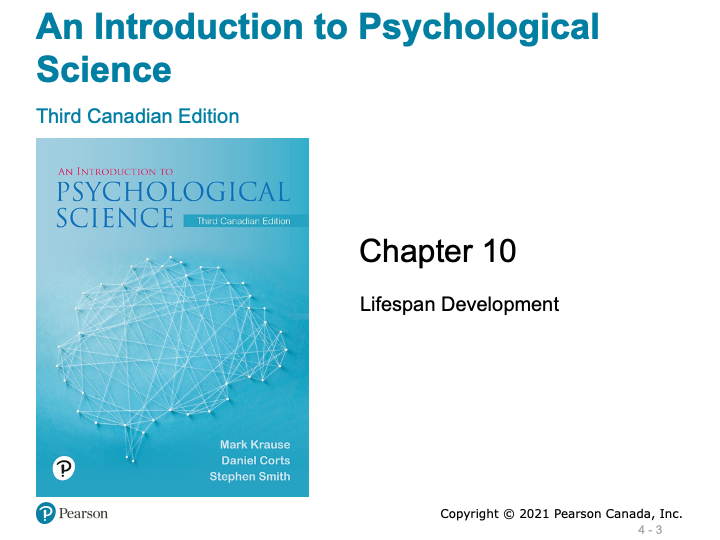
\includegraphics{assets/unit_3/slide_3.png}

\emph{Slide showing - Introduction}

Modules

\begin{itemize}
\tightlist
\item
  Physical Development from Conception through Infancy\\
\item
  Infancy and Childhood: Cognitive and Emotional Development\\
\item
  Adolescence\\
\item
  Adulthood and Aging
\end{itemize}

Learning Objectivess

\begin{itemize}
\tightlist
\item
  Know the key terminology related to prenatal and infant physical development.\\
\item
  Understand pros and cons to different research designs in developmental psychology.\\
\item
  Apply your understanding to identify the best ways expectant parents can ensure the health of their developing fetus.\\
\item
  Analyze the effects of preterm birth.
\end{itemize}

Developmental Psychology

\begin{itemize}
\tightlist
\item
  Developmental psychology (p.~362)

  \begin{itemize}
  \tightlist
  \item
    Early development influences later behaviours
  \end{itemize}
\end{itemize}

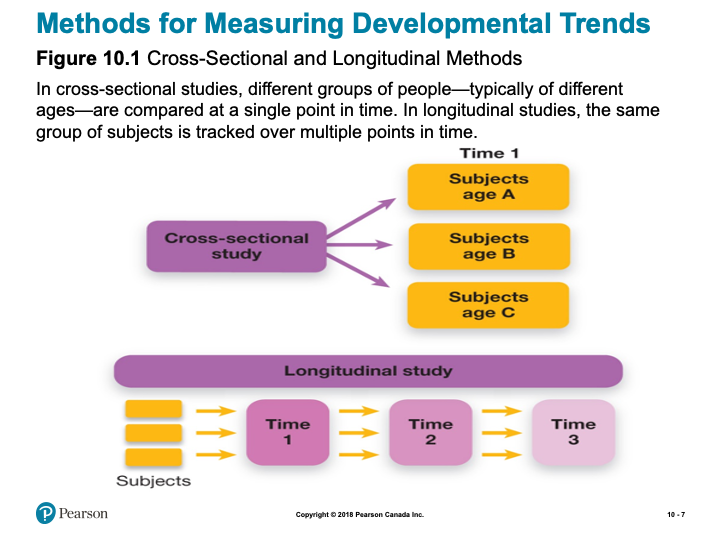
\includegraphics{assets/unit_3/slide_7.png}

\emph{Slide showing - Cross-Sectional and Longitudinal Methods}

Patterns of Development: Stages and Continuity

\begin{itemize}
\tightlist
\item
  Stages

  \begin{itemize}
  \tightlist
  \item
    Abrupt transitions\\
  \end{itemize}
\item
  Continuous

  \begin{itemize}
  \tightlist
  \item
    Slow changes
  \end{itemize}
\end{itemize}

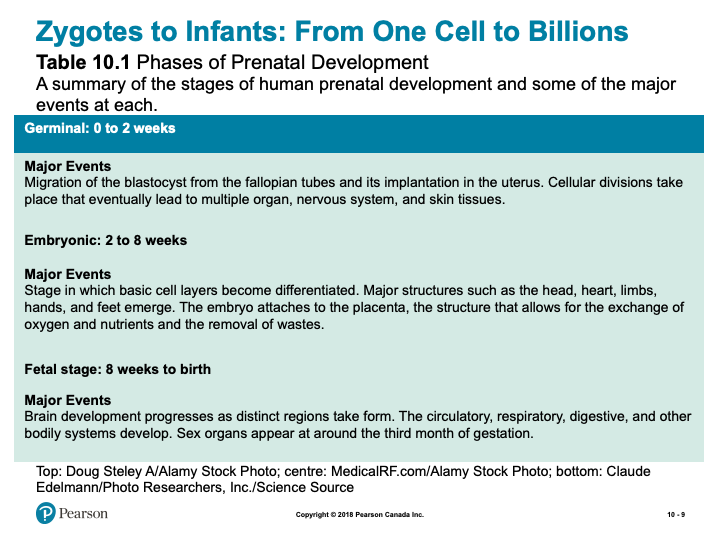
\includegraphics{assets/unit_3/slide_9.png}

\emph{Slide showing - Phases of Prenatal Development}

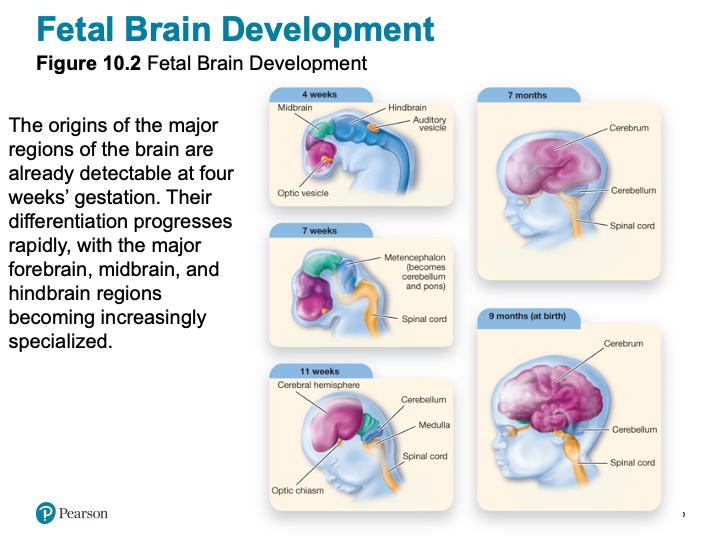
\includegraphics{assets/unit_3/slide_10.png}

\emph{Slide showing - Fetal Brain Development}

Nutrition, Teratogens, and Fetal Development

\begin{itemize}
\tightlist
\item
  Teratogen (p.~366)

  \begin{itemize}
  \tightlist
  \item
    Alcohol\\
  \item
    Cigarettes\\
  \end{itemize}
\item
  Fetal Alcohol Syndrome (p.~366)

  \begin{itemize}
  \tightlist
  \item
    1.5 in 1000 worldwide

    \begin{itemize}
    \tightlist
    \item
      Likely higher\\
    \end{itemize}
  \end{itemize}
\item
  Stress
\end{itemize}

Working the Scientific Literacy Model: The Long-Term Effects of Premature Birth (1 of 2)

\begin{itemize}
\tightlist
\item
  What do we know about premature birth?

  \begin{itemize}
  \tightlist
  \item
    Preterm infants (p.~368)\\
  \item
    25 weeks: 50\% survival\\
  \item
    30 weeks: 95\% survival\\
  \end{itemize}
\item
  How can science be used to help preterm infants?

  \begin{itemize}
  \tightlist
  \item
    NIDCAP
  \end{itemize}
\end{itemize}

Working the Scientific Literacy Model: The Long-Term Effects of Premature Birth (2 of 2)

\begin{itemize}
\tightlist
\item
  Can we critically evaluate this research?

  \begin{itemize}
  \tightlist
  \item
    Small sample size\\
  \item
    Why does the program work?\\
  \end{itemize}
\item
  Why is this relevant?

  \begin{itemize}
  \tightlist
  \item
    9\% of infants are born preterm\\
  \item
    Simple interventions available:

    \begin{itemize}
    \tightlist
    \item
      Massage\\
    \item
      Kangaroo care
    \end{itemize}
  \end{itemize}
\end{itemize}

Myths in Mind: Vaccinations and Autism

\begin{itemize}
\tightlist
\item
  1990 claim that MMR vaccine linked to autism

  \begin{itemize}
  \tightlist
  \item
    One dose given at year 1\\
  \item
    Second does before starting school\\
  \item
    Many parents refused\\
  \end{itemize}
\item
  Lack of scientific support

  \begin{itemize}
  \tightlist
  \item
    Article retracted 2010
  \end{itemize}
\end{itemize}

Sensory Development in Infancy

\begin{itemize}
\tightlist
\item
  Sensory before birth

  \begin{itemize}
  \tightlist
  \item
    4 months gestation, brain receiving signals from eyes and ears\\
  \item
    7-8 months gestation, fetus actively listening\\
  \end{itemize}
\item
  Vision at birth

  \begin{itemize}
  \tightlist
  \item
    30 cm or less\\
  \item
    20/20 by 12 months\\
  \end{itemize}
\item
  Smell at birth

  \begin{itemize}
  \tightlist
  \item
    Cringe at foul odours\\
  \item
    Discriminate mother's breastmilk
  \end{itemize}
\end{itemize}

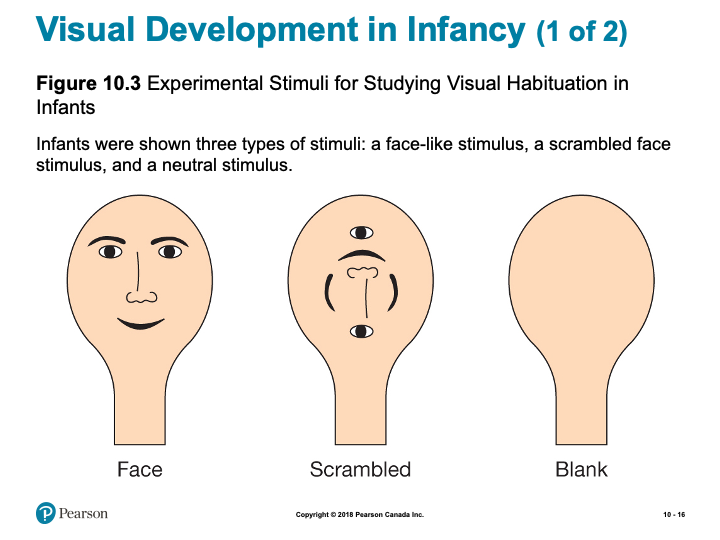
\includegraphics{assets/unit_3/slide_16.png}

\emph{Slide showing - Experimental Stimuli for Studying Visual Habituation in Infants}

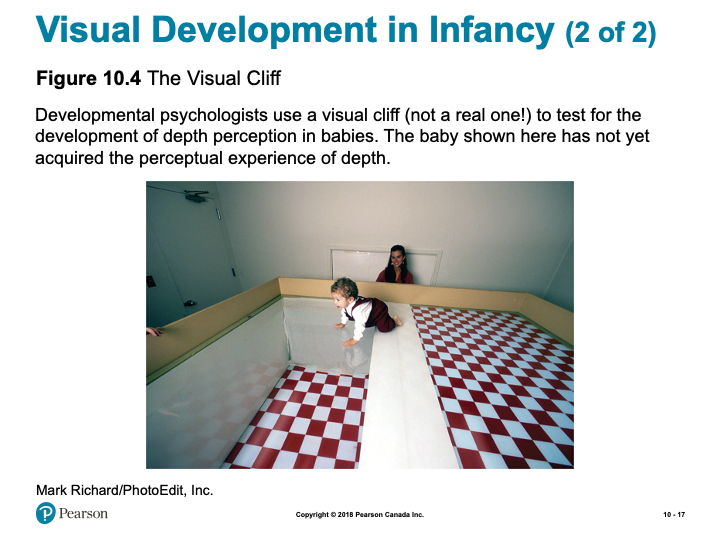
\includegraphics{assets/unit_3/slide_17.png}

\emph{Slide showing - The Visual Cliff}

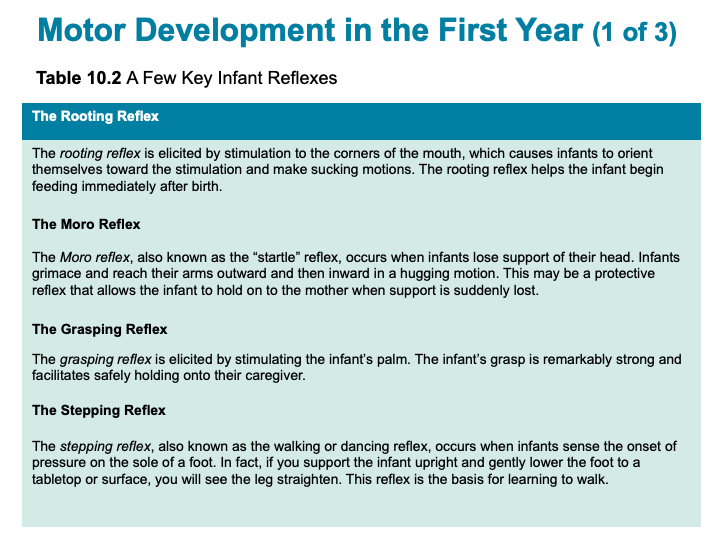
\includegraphics{assets/unit_3/slide_18.png}

\emph{Slide showing - A Few Key Infant Reflexes}

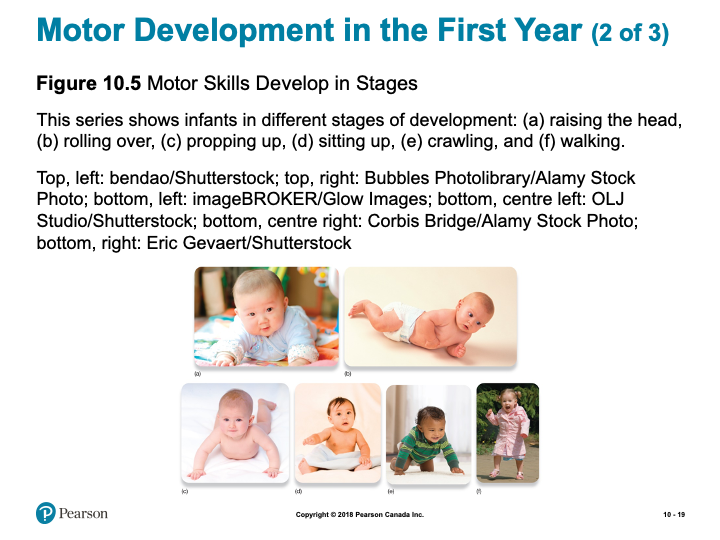
\includegraphics{assets/unit_3/slide_19.png}

\emph{Slide showing - Motor Skills Develop in Stages}

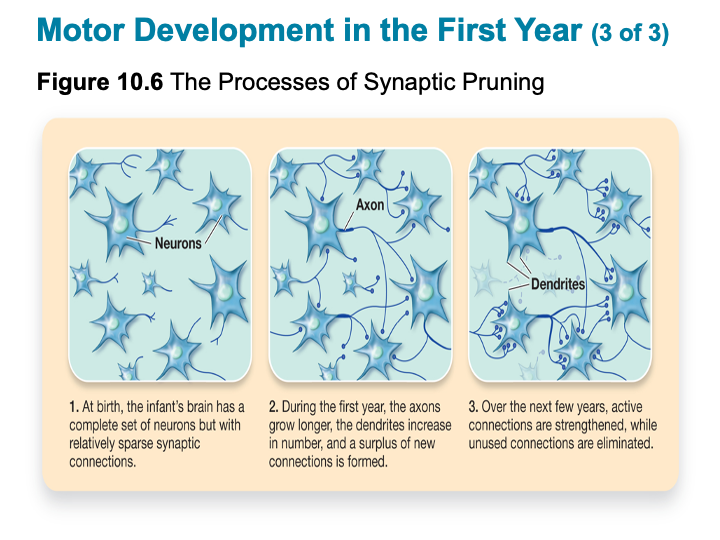
\includegraphics{assets/unit_3/slide_20.png}

\emph{Slide showing - The Processes of Synaptic Pruning}

Learning Objectives

\begin{itemize}
\tightlist
\item
  Know the key terminology associated with infancy and childhood.\\
\item
  Understand the cognitive changes that occur during infancy and childhood.\\
\item
  Understand the importance of attachment and the different styles of attachment.\\
\item
  Apply the concept of scaffolding and the zone of proximal development to understand how to best promote learning.\\
\item
  Analyze how to effectively discipline children in order to promote moral behaviour.
\end{itemize}

The Importance of Sensitive Periods

\begin{itemize}
\tightlist
\item
  Sensitive period (p.~375)

  \begin{itemize}
  \tightlist
  \item
    Language fluency\\
  \item
    Perception\\
  \item
    Balance\\
  \item
    Recognition of parents\\
  \item
    Identifying with a particular culture
  \end{itemize}
\end{itemize}

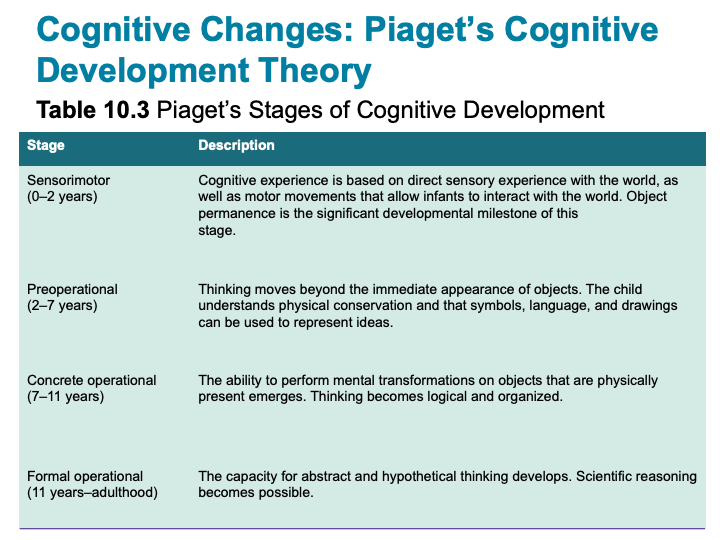
\includegraphics{assets/unit_3/slide_23.png}

\emph{Slide showing - Piaget's Stages of Cognitive Development}

The Sensorimotor Stage: Objects and the Physical World

\begin{itemize}
\tightlist
\item
  Sensorimotor stage (p.~375)

  \begin{itemize}
  \tightlist
  \item
    Birth to 2 years\\
  \item
    Object permanence (p.~376)

    \begin{itemize}
    \tightlist
    \item
      Hidden toy test
    \end{itemize}
  \end{itemize}
\end{itemize}

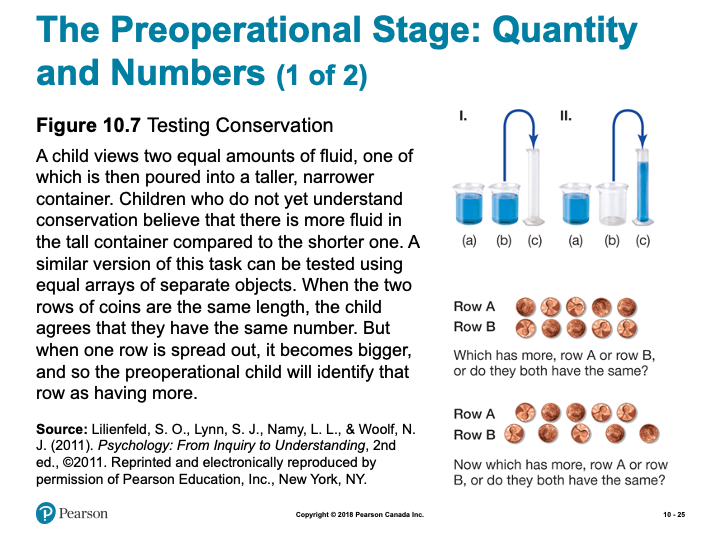
\includegraphics{assets/unit_3/slide_25.png}

\emph{Slide showing - Testing Conservation}

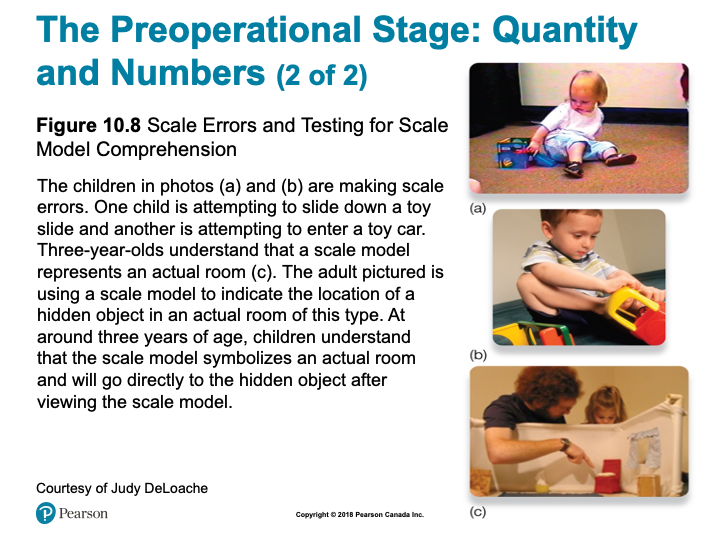
\includegraphics{assets/unit_3/slide_26.png}

\emph{Slide showing - Scale Errors and Testing for Scale Model Comprehension}

The Concrete Operational Stage: Using Logical Thought

\begin{itemize}
\tightlist
\item
  Concrete operational stage (p.~377)

  \begin{itemize}
  \tightlist
  \item
    7 to 11 years\\
  \item
    Transitivity
  \end{itemize}
\end{itemize}

The Formal Operational Stage: Abstract and Hypothetical Thought

\begin{itemize}
\tightlist
\item
  Formal operational stage (p.~378)

  \begin{itemize}
  \tightlist
  \item
    11 years to adulthood\\
  \item
    Scientific thinking
  \end{itemize}
\end{itemize}

Working the Scientific Literacy Model: Evaluating Piaget (1 of 3)

\begin{itemize}
\tightlist
\item
  What do we know about cognitive abilities in infants?

  \begin{itemize}
  \tightlist
  \item
    Core knowledge hypothesis (p.~378)\\
  \item
    Habituation (p.~378)\\
  \item
    Dishabituation (p.~378)
  \end{itemize}
\end{itemize}

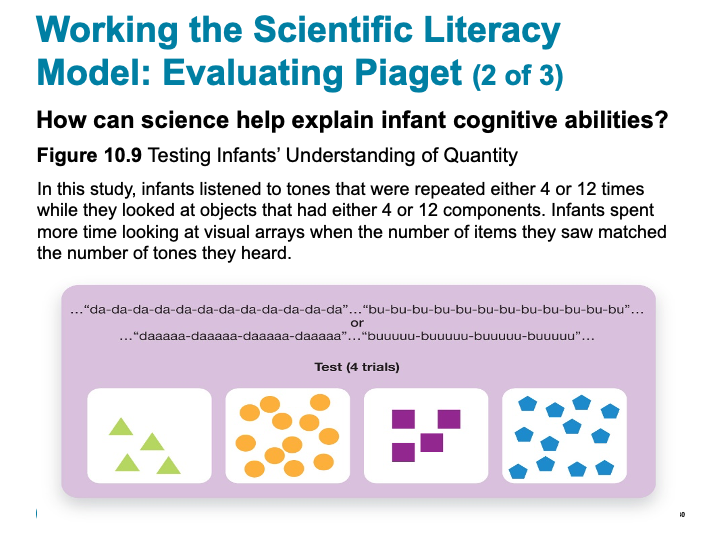
\includegraphics{assets/unit_3/slide_31.png}

\emph{Slide showing - Testing Infants' Understanding of Quantity}

Complementary Approaches to Piaget

\begin{itemize}
\tightlist
\item
  Vygotsky

  \begin{itemize}
  \tightlist
  \item
    Zone of proximal development (p.~380)

    \begin{itemize}
    \tightlist
    \item
      Scaffolding (p.~380)

      \begin{itemize}
      \tightlist
      \item
        Cultural differences
      \end{itemize}
    \end{itemize}
  \end{itemize}
\end{itemize}

Social Development and Attachment (1 of 2)

\begin{itemize}
\tightlist
\item
  Attachment (p.~381)\\
\item
  Harry Harlow's monkey experiments\\
\item
  Strange situation test (p.382)
\end{itemize}

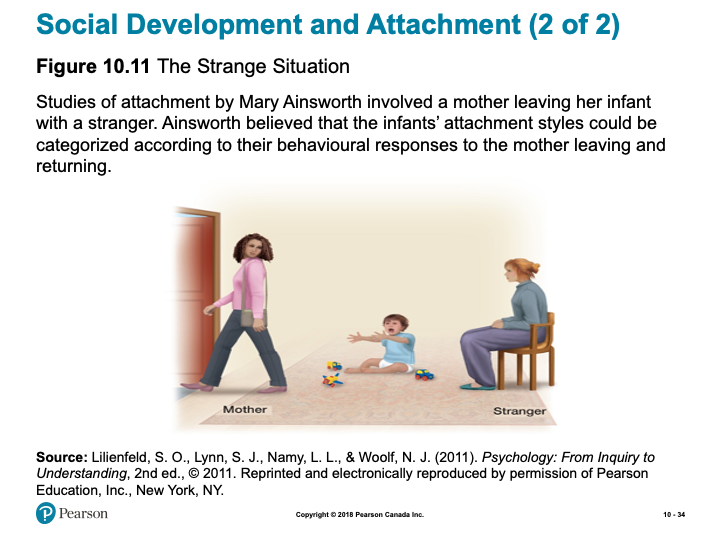
\includegraphics{assets/unit_3/slide_34.png}

\emph{Slide showing - The Strange Situation}

Social Development and Attachment (1 of 2)

\begin{itemize}
\tightlist
\item
  Types of Attachment\\
\item
  Secure attachment

  \begin{itemize}
  \tightlist
  \item
    Insecure attachment\\
  \item
    Disorganized\\
  \item
    Anxious/Ambivalent\\
  \item
    Avoidant
  \end{itemize}
\end{itemize}

Social Development and Attachment (1 of 2)

\begin{itemize}
\tightlist
\item
  Parenting and Attachment\\
\item
  Attachment behavioural system (p.~383)\\
\item
  Caregiving behavioural system (p.~383)\\
\item
  Conditional approaches\\
\item
  Introjection (p.~383)\\
\item
  Inductive discipline (p.~383)
\end{itemize}

Self-Awareness (1 of 3)

\begin{itemize}
\tightlist
\item
  Self-awareness (p.~384)

  \begin{itemize}
  \tightlist
  \item
    Reflection in mirror\\
  \end{itemize}
\item
  Egocentric (p.~384)
\end{itemize}

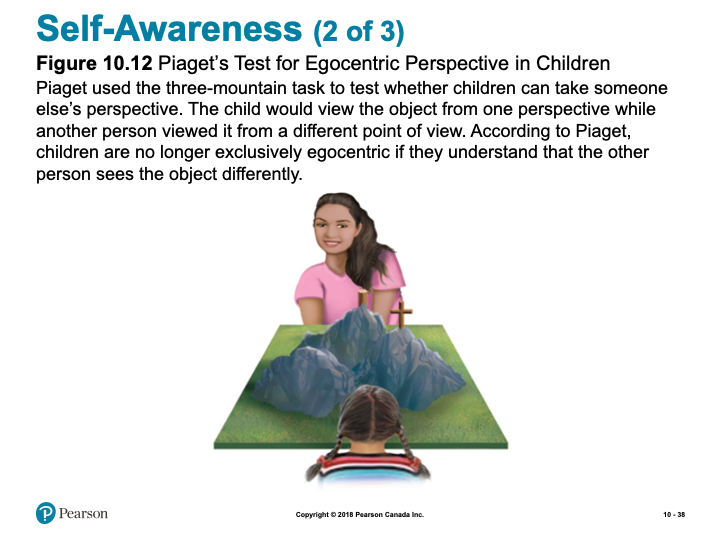
\includegraphics{assets/unit_3/slide_38.png}

\emph{Slide showing - Piaget's Test for Egocentric Perspective in Children}

Self-Awareness (3 of 3)

\begin{itemize}
\tightlist
\item
  Theory of mind (p.~384)\\
\item
  False-belief task
\end{itemize}

Psychosocial Development Across the Lifespan (1 of 2)

\begin{itemize}
\tightlist
\item
  Infancy

  \begin{itemize}
  \tightlist
  \item
    Sense of security\\
  \end{itemize}
\item
  Toddlerhood

  \begin{itemize}
  \tightlist
  \item
    Exploring autonomy\\
  \end{itemize}
\item
  Early Childhood

  \begin{itemize}
  \tightlist
  \item
    Pushing boundaries and experimenting\\
  \end{itemize}
\item
  Childhood

  \begin{itemize}
  \tightlist
  \item
    Active engagement
  \end{itemize}
\end{itemize}

10.3 Learning Objectives

\begin{itemize}
\tightlist
\item
  Know the key terminology concerning adolescent development.\\
\item
  Understand the process of identity formation during adolescence.\\
\item
  Understand the importance of relationships in adolescence.\\
\item
  Understand the functions of moral emotions.\\
\item
  Apply your understanding of the categories of moral reasoning.\\
\item
  Analyze the relationship between brain development and adolescent judgment and risk taking.
\end{itemize}

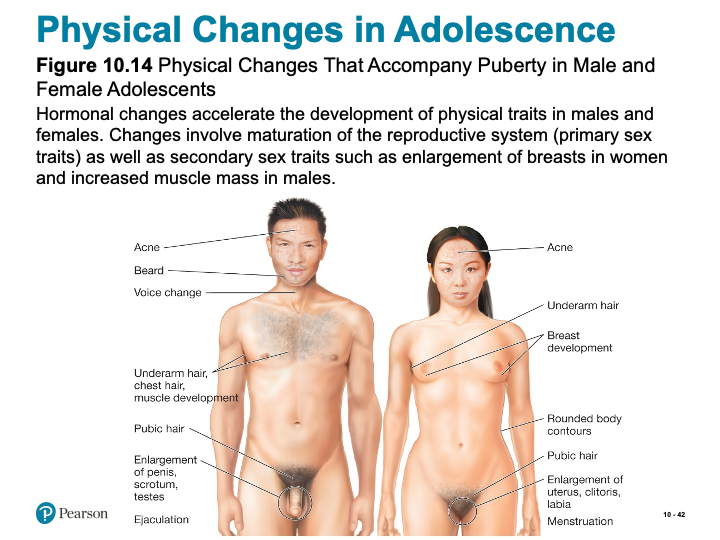
\includegraphics{assets/unit_3/slide_42.png}

\emph{Slide showing - Physical Changes That Accompany Puberty in Male and Female Adolescents}

Emotional Challenges in Adolescence

\begin{itemize}
\tightlist
\item
  Intense and volatile emotions\\
\item
  Cognitive reframing\\
\item
  Ability to delay gratification (p.~392)
\end{itemize}

Working the Scientific Literacy Model: Adolescent Risk and Decision Making (1 of 4)

\begin{itemize}
\tightlist
\item
  What do we know about adolescence and decision making?

  \begin{itemize}
  \tightlist
  \item
    Ongoing changes in prefrontal cortex

    \begin{itemize}
    \tightlist
    \item
      Region involved in impulse control, mood, planning, organizing, and reasoning
    \end{itemize}
  \end{itemize}
\end{itemize}

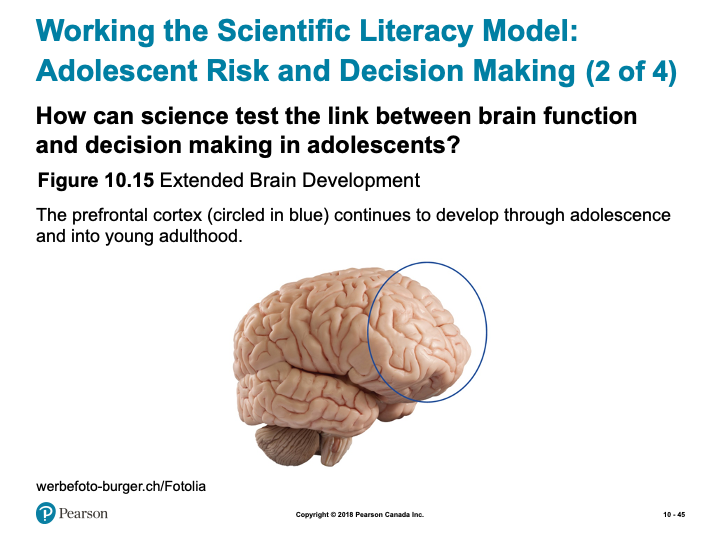
\includegraphics{assets/unit_3/slide_45.png}

\emph{Slide showing - Extended Brain Development}

Working the Scientific Literacy Model: Adolescent Risk and Decision Making (3 of 4)

\begin{itemize}
\tightlist
\item
  Can we critically evaluate this explanation for risky decision making?

  \begin{itemize}
  \tightlist
  \item
    Still capable of making good decisions\\
  \item
    Temperament and personality\\
  \item
    Situational factors\\
  \end{itemize}
\item
  Why is this relevant?

  \begin{itemize}
  \tightlist
  \item
    Major public health problem
  \end{itemize}
\end{itemize}

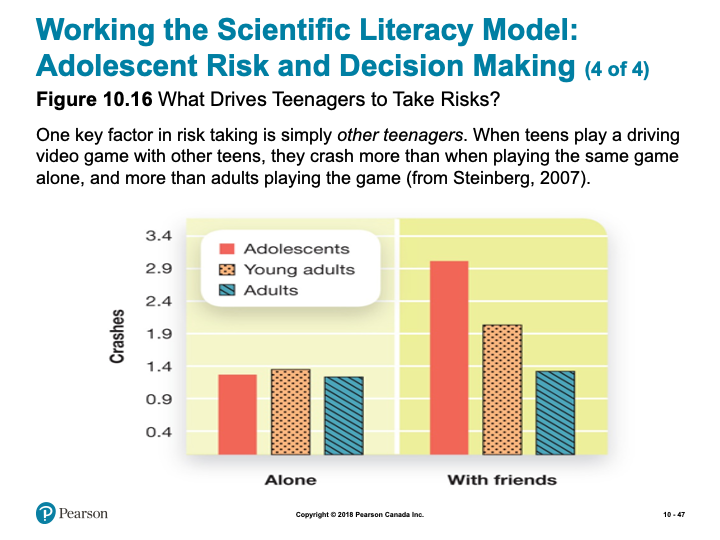
\includegraphics{assets/unit_3/slide_47.png}

\emph{Slide showing - What Drives Teenagers to Take Risks?}

Cognitive Development: Moral Reasoning vs.~Emotions

\begin{itemize}
\tightlist
\item
  Formal operational stage

  \begin{itemize}
  \tightlist
  \item
    Abstract thinking\\
  \item
    Scientific thinking\\
  \item
    Perspective taking
  \end{itemize}
\end{itemize}

Kohlberg's Moral Development: Learning Right from Wrong (1 of 2)

\begin{itemize}
\tightlist
\item
  A trolley is hurtling down the tracks toward a group of five unsuspecting people. You are standing next to a lever that, if pulled, would direct the trolley onto another track, thereby saving the five individuals. However, on the second track stands a single, unsuspecting person, who would be struck by the diverted trolley.
\end{itemize}

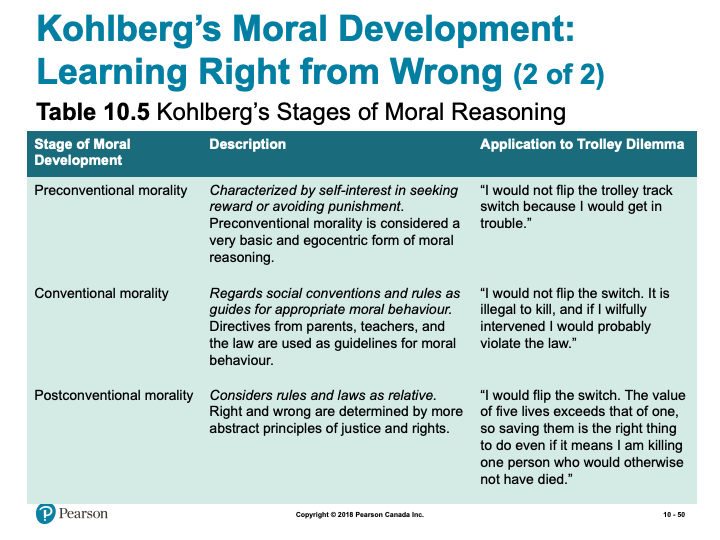
\includegraphics{assets/unit_3/slide_50.png}

\emph{Slide showing - Kohlberg's Stages of Moral Reasoning}

Moral Development

\begin{itemize}
\tightlist
\item
  Social intuitionist model

  \begin{itemize}
  \tightlist
  \item
    Julie and Steven are brother and sister. They are travelling together in France on summer vacation from college. One night they are staying alone in a cabin near the beach. They decide that it would be interesting and fun if they shared a romantic kiss. At the very least it would be a new experience for each of them. They both enjoy the experience, but they decide not to do it again. They keep that night as a special secret, which makes them feel even closer to each other.
  \end{itemize}
\end{itemize}

Social Development: Identity and Relationships

\begin{itemize}
\tightlist
\item
  Identity (p.~395)

  \begin{itemize}
  \tightlist
  \item
    Personal qualities\\
  \item
    Social qualities\\
  \item
    Future goals\\
  \end{itemize}
\item
  Adolescence identity crisis

  \begin{itemize}
  \tightlist
  \item
    Curiosity, questioning, and exploration\\
  \end{itemize}
\item
  Peer groups\\
\item
  Romantic relationships
\end{itemize}

10.4 Learning Objectives

\begin{itemize}
\tightlist
\item
  Know the key terminology concerning adulthood and aging.\\
\item
  Know the key areas of growth experiences by emerging adults.\\
\item
  Understand age-related disorders such as Alzheimer's disease.\\
\item
  Understand how cognitive abilities change with age.\\
\item
  Apply your attitudes about marriage.\\
\item
  Analyze the stereotype that old age is a time of unhappiness.
\end{itemize}

Physical Changes in Adulthood

\begin{itemize}
\tightlist
\item
  Age brackets:

  \begin{itemize}
  \tightlist
  \item
    Young adulthood: 18-40 years\\
  \item
    Middle adulthood: 40-65 years\\
  \item
    Older adulthood: 65 years and onward\\
  \end{itemize}
\item
  Menopause (p.~399)
\end{itemize}

Psychosocial Development Across the Lifespan (2 of 2)

\begin{itemize}
\tightlist
\item
  Ages 25 to 40

  \begin{itemize}
  \tightlist
  \item
    Separate from parents
  \item
    Work on intimate relationships
  \item
    Failure can result in isolation
  \end{itemize}
\item
  Ages 45 to 65
\item
  Producing something of value
\item
  Work and/or family
\item
  Ages 65+
\item
  Reflect on life of fulfillment (or not)
\end{itemize}

Love and Marriage

\begin{itemize}
\tightlist
\item
  Most adults pursue some kind of long-term relationship
\item
  Marriage associated with longer life, happiness
\item
  Gottman

  \begin{itemize}
  \tightlist
  \item
    Conflict and communication
  \item
    ``Four horsemen of the Apocalypse''
  \end{itemize}
\end{itemize}

Parenting

\begin{itemize}
\tightlist
\item
  Shift in identity, lifestyle
\item
  Children affect marriage
\item
  Empty nest myth
\end{itemize}

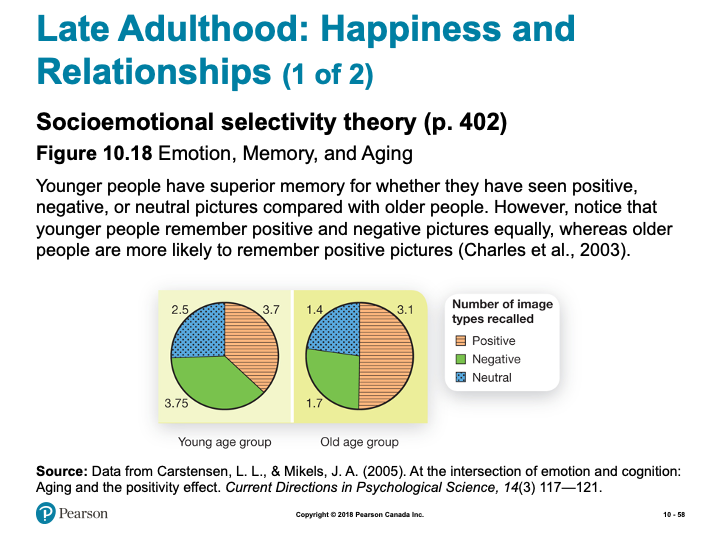
\includegraphics{assets/unit_3/slide_58.png}

\emph{Slide showing - Emotion, Memory, and Aging}

PSYCH @ The Driver's Seat

\begin{itemize}
\tightlist
\item
  Driving skills and age
\item
  UFOV Speed of Processing training

  \begin{itemize}
  \tightlist
  \item
    Computer-based
  \item
    Decreases accident risk
  \end{itemize}
\end{itemize}

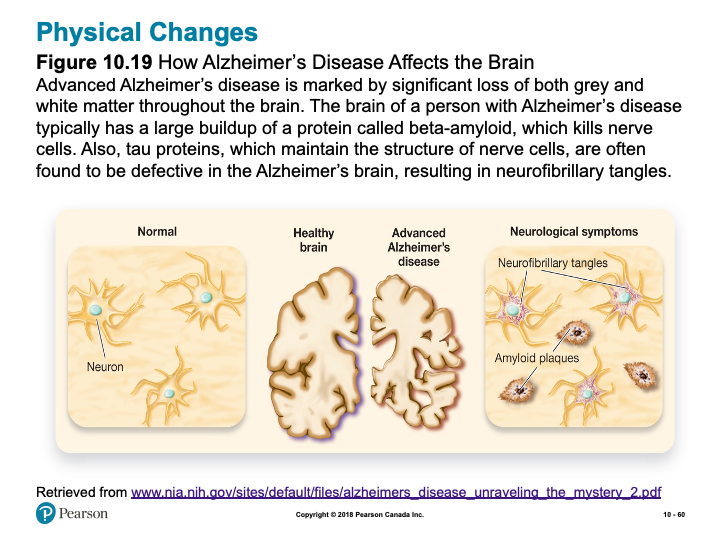
\includegraphics{assets/unit_3/slide_60.png}

\emph{Slide showing - How Alzheimer's Disease Affects the Brain}

Working the Scientific Literacy Model: Aging and Cognitive Change (1 of 3)

\begin{itemize}
\tightlist
\item
  What do we know about cognitive abilities?

  \begin{itemize}
  \tightlist
  \item
    Fluid intelligence declines
  \item
    Crystalized intelligence remains largely intact
  \end{itemize}
\item
  How can science explain age-related differences in cognitive abilities?

  \begin{itemize}
  \tightlist
  \item
    Activation of brain areas
  \end{itemize}
\end{itemize}

Working the Scientific Literacy Model: Aging and Cognitive Change (2 of 3)

\begin{itemize}
\tightlist
\item
  Can we critically evaluate our assumptions about age-related cognitive changes?

  \begin{itemize}
  \tightlist
  \item
    Too simplistic to say memory declines

    \begin{itemize}
    \tightlist
    \item
      Many different types of memory
    \end{itemize}
  \item
    Compensation
  \end{itemize}
\item
  Why is this relevant?

  \begin{itemize}
  \tightlist
  \item
    Control over how one ages
  \end{itemize}
\end{itemize}

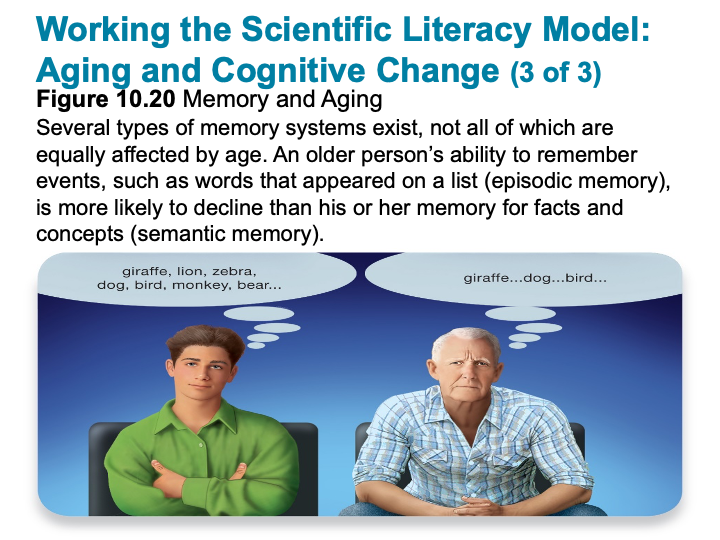
\includegraphics{assets/unit_3/slide_63.png}

\emph{Slide showing - Memory and Aging}

\textbf{Note:} The slides are intended to supplement the information found in your textbook. If you are having trouble viewing them, they can also be downloaded by scrolling to the bottom of the screen and clicking on the ``Unit 3 - Slides'' link.

\textbf{Designer Babies}

\begin{itemize}
\tightlist
\item
  Explore and reflect upon this contemporary and controversial issue. Designer babies pose many ethical issues and requires careful consideration.
\end{itemize}

\textbf{Cognitive Change}

\begin{itemize}
\tightlist
\item
  Reflect on your own development before taking a ``test'' to develop additional insights into your own developmental trajectory.
\end{itemize}

\textbf{Terminology Practice}

\begin{itemize}
\tightlist
\item
  Take this flip-card activity to self-evaluate how well you know some of the important terms from Chapter 10.
\end{itemize}

\textbf{\emph{Learning Lab Preparation}}

\begin{itemize}
\tightlist
\item
  Each topic will provide a question or scenario for you to consider prior to attending your Learning Lab. Be sure to carefully consider each prompt as you will be expected to contribute to the group discussion.
\end{itemize}
\end{reflect}

\hypertarget{resources}{%
\subsection*{Resources}\label{resources}}
\addcontentsline{toc}{subsection}{Resources}

Here are some additional resources that will help you complete this unit:

\begin{itemize}
\tightlist
\item
  Krause, M., Corts, D., Smith, S. C., \& Dolderman, D. (2018). \emph{Revel for An Introduction to Psychological Science, 2nd Canadian Edition.} Pearson Ed.\\
\item
  Other resources will be provided online.
\end{itemize}

\hypertarget{prenatal-development}{%
\section{Prenatal Development}\label{prenatal-development}}

\hypertarget{physical-development}{%
\subsection*{Physical Development}\label{physical-development}}
\addcontentsline{toc}{subsection}{Physical Development}

Prenatal development is a time of rapid growth and change. This rapid change continues throughout the first few years of life. Development during early life is clearly a function both of nature and of the environment.

\textbf{\emph{Questions to Consider}}

After you have read the first few pages of this chapter you should be able to answer the following questions:

\begin{itemize}
\tightlist
\item
  \textbf{\emph{How is the gender of an offspring determined?}}
\item
  \textbf{\emph{What differentiates zygotes from embryos and embryos from fetuses?}}
\end{itemize}

\emph{(These questions are intended for personal reflection - you are not intended to submit anything for assessment)}

\hypertarget{designer-babies}{%
\subsection*{Designer Babies}\label{designer-babies}}
\addcontentsline{toc}{subsection}{Designer Babies}

It is beginning to look inevitable that, however fierce the debate, the technology to make designer babies will happen - maybe just 20 years from now. Geneticists claim to have found the gene for good-parenting, genes for obesity, Alzheimer's, red hair, and even happiness. Incredibly, scientists have even constructed an artificial human chromosome, which could carry any genes a geneticist - or prospective parents - desired.

Embryo A technique called Pre-implantation Genetic Diagnosis (PGD) is already being used to screen embryos for genetic diseases. Embryos created outside the body using in vitro fertilization are tested to see whether they carry a genetic disorder before being transferred to the uterus. It's deeply controversial whether parents should ever be allowed to select embryos just because they're genetically different.

At the moment the technique is used for therapeutic purposes only, to screen for children who may have a deadly genetic disease. Even if some parents and their doctors were willing to use PGD for cosmetic or enhancement purposes, which remains absolutely taboo, the technique is limited in a crucial way - PGD can only select an embryo with genes inherited from the parents.

\textbf{\emph{Bottled Genes?}} \emph{One day parents may be able to pick any gene they desire from a range of bottled genes and have it put into their embryos. (quoted from ``Designer Babies'' website)}

\hypertarget{learning-activities}{%
\subsection*{Learning Activities}\label{learning-activities}}
\addcontentsline{toc}{subsection}{Learning Activities}

\hypertarget{designer-babies-1}{%
\subsubsection*{Designer Babies}\label{designer-babies-1}}
\addcontentsline{toc}{subsubsection}{Designer Babies}

This activity involves some reading and reflection around the topic of genetic engineering. As this is a contemporary issue, it will be valuable to familiarize yourself with some of the complexities of this technology and think critically about some of the ethical challenges. Your task is to read the following resources and carefully consider the implications of this technology:

\begin{itemize}
\tightlist
\item
  \href{https://www.statnews.com/2019/09/16/could-editing-the-dna-of-embryos-with-crispr-help-save-people-who-are-already-alive/}{\textbf{Editing the DNA of Embryos with CRISPR}}\\
\item
  \href{https://www.geneticsandsociety.org/internal-content/designer-babies-crispr-genetic-engineering}{\textbf{Designer Babies, CRISPR, \& Genetic Engineering}}
\end{itemize}

\hypertarget{learning-lab-preparation}{%
\subsubsection*{Learning Lab Preparation}\label{learning-lab-preparation}}
\addcontentsline{toc}{subsubsection}{Learning Lab Preparation}

Prior to your Learning Lab, take some time to think about the following scenario and questions. You will be asked to share your thoughts in this week's Learning Lab:

\emph{Modern techniques of conception and human genetic engineer­ing raise important new issues for human development. A pam­phlet containing the following message was left at doorsteps in TWU professor Philipchalk's neighborhood:}

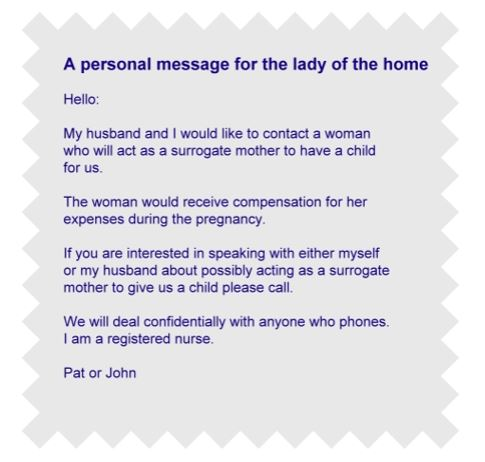
\includegraphics{assets/unit_3/U3_T1_LearningACtivitity.JPG}

\emph{Image showing an example of surrogacy message }

(\emph{You may also wish to comment on the ``Designer Babies'' topic above.})

\begin{enumerate}
\def\labelenumi{\arabic{enumi}.}
\tightlist
\item
  \textbf{\emph{How do you feel about this request?}}
\item
  \textbf{\emph{What problems might you anticipate?}}
\end{enumerate}

\hypertarget{infancy-and-childhood}{%
\section{\texorpdfstring{\textbf{Infancy and Childhood}}{Infancy and Childhood}}\label{infancy-and-childhood}}

\hypertarget{a-childs-view-of-god}{%
\subsection*{A Child's View of God}\label{a-childs-view-of-god}}
\addcontentsline{toc}{subsection}{A Child's View of God}

One evening on a camping trip several years ago, my wife and I listened outside the tent as our five-year-old Joelle and three-year-old Matthew tried to get to sleep. Always the ``mother,'' Joelle attempted to dispel her little brother's fear of bears and other wild creatures by reminding him that Jesus was watching over them. Not content with generalities, Matt responded, ``Does Jesus got a gun?'' \emph{(Psychology and Christianity by Ronald Philipchalk, p.~141)}

As any Sunday School teacher knows, children see God differently from adults---often in very concrete terms (protection requires a gun!). Studying cognitive development can help us to understand as well as teach children at their own level.

\hypertarget{the-process-of-cognitive-change}{%
\subsection*{The Process of Cognitive Change}\label{the-process-of-cognitive-change}}
\addcontentsline{toc}{subsection}{The Process of Cognitive Change}

Our textbook provides a good summary of the structure (stages) of cognitive development. The section, however, does not address the process by which a person moves from one stage to the next. Piaget believed that the key to cognitive development is something called cognitive conflict or cognitive disequilibrium. For cognitive development to proceed, the individual must constantly re-evaluate his or her schemas. According to Piaget, we develop schemas from an early age of life. Schemas are our cognitive representations of the world. Schemas help us to organize our experiences. They also allow us to make predictions about what outcomes might result from particular behaviours. Schemas are very important in helping us to understand and to adapt to the world.

Although schemas are important in helping us to understand the world, they are not always accurate. People at all ages can have mental representations of the world that are not correct.

\textbf{\emph{Can you think of any examples of inaccurate schemas?}}

Although people at all ages can have inaccurate mental representations of the world, children are especially prone to view the world in an incorrect way. The reason children may view the world in an incorrect way is because the structure of their cognitive processing is developing. Piaget believed that inaccurate schemas are changed only when they are challenged in the cognitive structure of the child. This challenge has been termed cognitive conflict.

Basically, the process of cognitive change works as follows:

\begin{itemize}
\tightlist
\item
  People are motivated to maintain a state of cognitive equilibrium.\\
\item
  When a child encounters information from the world and the information is inconsistent with his or her schema, the new piece of information creates a state of disequilibrium or cognitive conflict.\\
\item
  \textbf{\emph{Equilibrium}} may be restored through one of the two processes of adapation called assimilation and accommodation.\\
\item
  \textbf{\emph{Assimilation}} occurs when a child re-organizes the new information in such a way as to make the new piece of information consistent with his or her preexisting schema of the world.\\
\item
  \textbf{\emph{Accommodation}} occurs when a child alters his or her schema such that the new piece of information can now be incorporated into the new schema.
\end{itemize}

Thus the process of accommodation produces the greatest cognitive change. Can you think of examples of both assimilation and accommodation? Here is an example:

\textbf{Equilibrium-Preexisting Schema:} Child has grown up in an environment where all people he interacted with were of the same race (mom, dad, siblings, grandma, grandpa, etc.) Child has seen people of other racial groups, but has never interacted with them. Child develops the schema that people tend to like others who are of the same race as him or her.

\textbf{Cognitive Conflict Produced:} At four years of age the child begins to attend preschool. At this time he starts to interact with children of various races. The child begins to develop a friendship with a child of a different race. This friendship creates cognitive conflict for the child: ``How can I like someone who is a different color?'' To resolve this cognitive conflict, the child has two options:

\textbf{\emph{Option A}}- \textbf{Assimilation:} In order to maintain his or her preexisting schema, the child re-organizes the information such that the other child is not perceived to be so dissimilar after all: ``Maybe he is a different color from me, but we both speak English. We must not be so dissimilar after all.''

\textbf{\emph{Option B}}- \textbf{Accommodation:} The child's preexisting schema is altered such that the new information can be incorporated into a new way of perceiving the world, ``Maybe I can be friends with someone who is different from me.''

\hypertarget{cognitive-equilibrium-is-restored}{%
\subsection*{Cognitive Equilibrium is Restored}\label{cognitive-equilibrium-is-restored}}
\addcontentsline{toc}{subsection}{Cognitive Equilibrium is Restored}

Although cognitive equilibrium is restored via either assimilation or accommodation, assimilation serves to maintain an inaccurate schema (that differences inhibit the development of friendships) whereas accommodation serves to produce cognitive change and hence produces a more accurate representation of the world (that differences do not inhibit the development of friendships).

\hypertarget{learning-activities-1}{%
\subsection*{Learning Activities}\label{learning-activities-1}}
\addcontentsline{toc}{subsection}{Learning Activities}

\begin{reflect}
\hypertarget{cognitive-change}{%
\subsubsection*{Cognitive Change}\label{cognitive-change}}
\addcontentsline{toc}{subsubsection}{Cognitive Change}

The first three links below are articles that are intended to give you an opportunity to reflect upon your own considerations around development. The last link is a test - along with the first three links, it is intended to provide some insights about your developmental trajectory in light of your crisis resolution, attachment style, and parenting styles:

\begin{itemize}
\tightlist
\item
  \href{http://www.childdevelopmentinfo.com/development/erickson.shtml}{\textbf{Erik Erikson's Stages of Social-Emotional Development}}\\
\item
  \href{http://www.attachmentdisorder.net/}{\textbf{The Link Between Substance Abuse and Attachment Disorder}}\\
\item
  \href{https://www.mayoclinic.org/healthy-lifestyle/childrens-health/in-depth/stepfamilies/art-20047046}{\textbf{Stepfamilies: How to Help Your Child Adjust}}\\
\item
  \href{https://www.3smartcubes.com/pages/tests/parentingstyle/parentingstyle_instructions/}{\textbf{What is Your Parenting Style}}
\end{itemize}

\hypertarget{learning-lab-preparation-1}{%
\subsubsection*{Learning Lab Preparation}\label{learning-lab-preparation-1}}
\addcontentsline{toc}{subsubsection}{Learning Lab Preparation}

Prior to your Learning Lab, take some time to think about the following questions. You will be asked to share your thoughts in this week's Learning Lab:

\begin{itemize}
\tightlist
\item
  \textbf{\emph{What is God like for children of different levels of cognitive development? If you can, give some examples from children you know\ldots.}}
\item
  \textbf{\emph{Would children even have an idea of God if they were not taught it?}}
\end{itemize}
\end{reflect}

\hypertarget{adolescence}{%
\section{Adolescence}\label{adolescence}}

John has just turned 13. Over the past year he has experienced may changes. He has grown over six inches and he has developed acne over his face and back. Not only is he changing physically, he is also experiencing a wave of emotional, spiritual, cognitive, and sexual changes. John has become self-focused and very self-critical. In addition, he is beginning to think abstractly and to challenge adults' ``dominion'' on knowledge. John is also on a quest to understand ``who he is'' and ``what his place is in the world''. John's quest for an identity makes him more vulnerable to peer pressure and to the influence of radical groups and cults. During this time that we call adolescence, John will make many decisions that will have a profound effect on the direction his life will take.

\emph{Does any of the above sound familiar?}

Before you begin reading the textbook section on adolescence, think back to your own adolescence. As you think about your experience of adolescence, use the following questions to guide your reflection:

\begin{itemize}
\tightlist
\item
  What physical changes did you experience in adolescence?
\item
  How did these physical changes make you feel?
\item
  In what ways did your view of the world change during adolescence?
\item
  How did your way of treating other people change during adolescence?
\item
  What was most important to you during adolescence?
\item
  To what extent is ``who you are today'' a function of ``who you became during adolescence''?
\end{itemize}

\hypertarget{no-adolescence}{%
\subsection*{No Adolescence?}\label{no-adolescence}}
\addcontentsline{toc}{subsection}{No Adolescence?}

In other times and in other cultures to­day, adolescence does not exist as a significant and distinct period of develop­ment. This might seem surprising and difficult to imagine. Think of how modern society would be different, or if it could even exist, without a period of adolescence. What are the advantages and disadvantages of having an adolescent period?

\hypertarget{identity}{%
\subsection*{Identity}\label{identity}}
\addcontentsline{toc}{subsection}{Identity}

The concept of identity is a rich topic for consideration. The most familiar aspect of identity is occupational identity, since much of ``who we are'' in our society rests on the kind of work we do. Perhaps you can readily relate to this in your choice of major. Less familiar, but equally important, is ideological identity. Ideologi­cal identity, including both religious and political orientations, may un­dergo a tremen­dous upheaval during your student years. Do you have the same political beliefs as your parents? What about religious beliefs? Conflict and questioning of parental beliefs and values may be a necessary part of establishing your personal iden­tity---even if the beliefs and values you ultimately adopt are the same as those of your parents.

\hypertarget{learning-activities-2}{%
\subsection*{Learning Activities}\label{learning-activities-2}}
\addcontentsline{toc}{subsection}{Learning Activities}

\begin{reflect}
\hypertarget{read-and-reflect}{%
\subsubsection*{Read and Reflect}\label{read-and-reflect}}
\addcontentsline{toc}{subsubsection}{Read and Reflect}

In this section we explore adolescence and the changes in development we go through. Below are some resources that help to help support your understanding:

\begin{itemize}
\tightlist
\item
  \href{https://www.sciencedirect.com/journal/journal-of-adolescence}{\textbf{Journal of Adolescence}}\\
\item
  \href{https://childdevelopmentinfo.com/child-development/erickson/\#gs.d8mpcv}{\textbf{Erik Erikson's Stages of Social-Emotional Development}}\\
\item
  \href{http://drjamesdobson.org/quiz/parenting-quiz/4-tips-for-parenting-teenagers}{\textbf{4 Tips for Parenting Teenagers}}
\end{itemize}

\hypertarget{terminology-practice}{%
\subsubsection*{Terminology Practice}\label{terminology-practice}}
\addcontentsline{toc}{subsubsection}{Terminology Practice}

In order to review some of the major terms from Chapter 10 in your textbook, practice using the activity below. Although you will not be evaluated on these terms, they will assist you in the assessments for this course:

\hypertarget{learning-lab-preparation-2}{%
\subsubsection*{Learning Lab Preparation}\label{learning-lab-preparation-2}}
\addcontentsline{toc}{subsubsection}{Learning Lab Preparation}

Prior to your Learning Lab, take some time to think about the following questions. You will be asked to share your thoughts in this week's Learning Lab:

\begin{itemize}
\tightlist
\item
  \textbf{\emph{Would you want to live your adolescence over again if you could? Why or why not?}}
\end{itemize}
\end{reflect}

\hypertarget{assessment}{%
\section*{Assessment}\label{assessment}}
\addcontentsline{toc}{section}{Assessment}

\begin{assessment}
While there is no ``formal'' assignment that you will be responsible for submitting for Unit 3, you will be expected to participate in discussion during your Learning Lab. Your facilitator will be providing a participation mark based on your contributions. Below is some information to consider prior to attending your Learning Lab:

\emph{Active participation in group exercises, reflection, and critical discourse is an essential component of this course. You are expected to show respect for all members of the course, both in your speech and actions. Contribute by actively observing and listening, raising thoughtful questions, examining relevant issues, building on others' ideas, analyzing and evaluating the group's thinking, synthesizing key points, and expanding the group's perspectives. Take care not to dominate a conversation, giving space for others to speak. When in small groups help maintain the focus, flow, and quality of conversations, and take the initiative to invite others (particularly those who are quiet) to speak.}

\textbf{Rubric for Participation in Learning Labs}

\begin{longtable}[]{@{}
  >{\raggedright\arraybackslash}p{(\columnwidth - 4\tabcolsep) * \real{0.3333}}
  >{\raggedright\arraybackslash}p{(\columnwidth - 4\tabcolsep) * \real{0.3333}}
  >{\raggedright\arraybackslash}p{(\columnwidth - 4\tabcolsep) * \real{0.3333}}@{}}
\toprule\noalign{}
\begin{minipage}[b]{\linewidth}\raggedright
Emerging (0-64\%)
\end{minipage} & \begin{minipage}[b]{\linewidth}\raggedright
Developing (65-89\%)
\end{minipage} & \begin{minipage}[b]{\linewidth}\raggedright
Mastering (90-100\%)
\end{minipage} \\
\midrule\noalign{}
\endhead
\bottomrule\noalign{}
\endlastfoot
Never to almost never: Demonstrates active listening (as indicated by disengaged body language and no to rare comments that build on others' remarks),Initiates any contributions in class or small groups, Makes insightful or constructive comments, Helps maintain a supportive space for others to speak. & Sometimes to fairly often: Demonstrates active listening (as indicated by somewhat to often engaged body language and comments that build on others' remarks), Initiates a contribution at least once in a class or small group discussion; Makes insightful or constructive comments, Helps maintain a supportive space for others to speak. & Very often to nearly always: Demonstrates active listening (as indicated by fully engaged body language and comments that build on others' remarks), Initiates more than one contribution in a class or small group discussion, Makes insightful or constructive comments, Creates a space for others to speak and takes initiative to include others. \\
\end{longtable}
\end{assessment}

\hypertarget{checking-your-learning}{%
\section*{Checking your Learning}\label{checking-your-learning}}
\addcontentsline{toc}{section}{Checking your Learning}

\begin{progress}
Before you move on to the next unit, check that you are able to:

\begin{itemize}
\tightlist
\item
  Define the key terminology related to prenatal and infant physical development, infancy and childhood, and adolescent development.\\
\item
  Understand advantages and disadvantages to different research designs in developmental psychology.\\
\item
  Understand the cognitive changes that occur during infancy and childhood, and the importance of attachment and the different styles of attachment.\\
\item
  Understand the process of identity formation, relationships, and moral emotions during adolescence.\\
\item
  Apply your understanding to identify the best ways expectant parents can ensure the health of their developing fetus, how to promote learning, and how to categorize moral reasoning.\\
\item
  Analyze the effects of preterm birth, how to effectively discipline children, and adolescent judgment and risk taking.
\end{itemize}
\end{progress}

\hypertarget{the-developing-person---part-2}{%
\chapter{The Developing Person - Part 2}\label{the-developing-person---part-2}}

\hypertarget{overview-1}{%
\section*{Overview}\label{overview-1}}
\addcontentsline{toc}{section}{Overview}

Building upon Unit 3, this unit (Part 2) will focus on the cognitive, physical, and social changes faced during young (and emerging) adulthood, middle adulthood, and late adulthood. \emph{Please note as well, that although it is not covered in the text, Topic 2 discusses the important, and inevitable, subject of dying and death.}

\hypertarget{topics-1}{%
\subsection*{Topics}\label{topics-1}}
\addcontentsline{toc}{subsection}{Topics}

This unit is divided into the following topics:

\begin{enumerate}
\def\labelenumi{\arabic{enumi}.}
\tightlist
\item
  Adulthood
\item
  Death and Dying
\end{enumerate}

\hypertarget{learning-outcomes-1}{%
\subsection*{Learning Outcomes}\label{learning-outcomes-1}}
\addcontentsline{toc}{subsection}{Learning Outcomes}

By the end of this unit, student's will be able to:

\begin{itemize}
\tightlist
\item
  Define the key terminology concerning adulthood and aging.
\item
  Describe the key areas of growth experiences by emerging adults.
\item
  Explain age-related disorders such as Alzheimer's disease.
\item
  Describe how cognitive abilities change with age.
\item
  Apply effective communication principles to the challenge of improving your own relationships.
\item
  Analyze the stereotype that old age is a time of unhappiness.
\end{itemize}

\hypertarget{activity-checklist-1}{%
\subsection*{Activity Checklist}\label{activity-checklist-1}}
\addcontentsline{toc}{subsection}{Activity Checklist}

Here is a checklist of learning activities you will benefit from in completing this unit. You may find it useful for planning your work:

\textless-~\href{_schedule}{plugin:content-inject} --\textgreater{}

\textbf{Read and Reflect}

\begin{itemize}
\tightlist
\item
  Read \emph{Krause et al.~(2021). Revel for An Introduction to Psychological Science, 3rd Canadian Edition}\\
\item
  Review \href{PSYC106-CH10LifespanDevelopment-3rdEd.pptx}{\emph{Unit 4 - Slides}}\\
\item
  Review \emph{Unit 4 - Slides}
\end{itemize}

CLICK HERE

Chapter 10 - Lifespan Development

Psalm 92:12-15

\begin{itemize}
\tightlist
\item
  \(\scriptstyle 12\) The righteous will flourish like a palm tree,they will grow like a cedar of Lebanon;
\item
  \(\scriptstyle 13\) planted in the house of the Lord,they will flourish in the courts of our God.
\item
  \(\scriptstyle 14\) They will still bear fruit in old age,~~~~they will stay fresh and green,
\item
  \(\scriptstyle 15\) proclaiming, ``The Lord is upright;~~~~he is my Rock, and there is no wickedness in him.''
  //todo \#3
\item
  Video: (Annie Murphy Paul: What we learn before we're born){[}\url{http://www.ted.com/talks/annie_murphy_paul_what_we_learn_before_we_re_born.html} {]}
\end{itemize}

10.1 Learning Objectives

\begin{itemize}
\tightlist
\item
  Know the key terminology related to prenatal and infant physical development.\\
\item
  Understand pros and cons to different research designs in developmental psychology.\\
\item
  Apply your understanding to identify the best ways expectant parents can ensure the health of their developing fetus.\\
\item
  Analyze the effects of preterm birth.
\end{itemize}

Developmental Psychology

\begin{itemize}
\tightlist
\item
  Developmental psychology (p.~362)\\
\item
  Early development influences later behaviours
\end{itemize}

Developmental Psychology

\textbf{Note:} the slides are intended to supplement the information found in your textbook. If you are having trouble viewing them, they can also be downloaded by scrolling to the bottom of the screen and clicking on the ``Unit 4 - Slides'' link.*

\textbf{Relationships and Aging}

\begin{itemize}
\tightlist
\item
  Read about Erikson's Eight Psychosocial Stages that highlight the importance of relationships in healthy aging.
\end{itemize}

\textbf{Death and Dying}

\begin{itemize}
\tightlist
\item
  Take a moment to read through some resources that are focused on aging and dying. These readings are intended to provoke thought around the inevitability of death.
\end{itemize}

\textbf{\emph{Learning Lab Preparation}}

\begin{itemize}
\tightlist
\item
  Each topic will provide a question or scenario for you to consider prior to attending your Learning Lab. Be sure to carefully consider each prompt as you will be expected to contribute to the group discussion.
\end{itemize}

\hypertarget{assessment-1}{%
\subsubsection*{Assessment}\label{assessment-1}}
\addcontentsline{toc}{subsubsection}{Assessment}

\begin{itemize}
\item
  At the end of this unit, not only will you be assessed on your participation during the Learning Lab discussions, but you will also be responsible for submitting your first writing assignment.
\item
  \textbf{\emph{Writing Assignment \#1}} is outlined on the ``Assessment'' page - expectations for this assignment, as well as a grading rubric, can be found by clicking on that tab.
\item
  After completing this assignment, you will also be expected to complete \textbf{\emph{Quiz \#1.}} Again, information about the quiz can be found by clicking on the ``Assessment'' tab.
\end{itemize}

\hypertarget{resources-1}{%
\subsection*{Resources}\label{resources-1}}
\addcontentsline{toc}{subsection}{Resources}

Here are some additional resources that will help you complete this unit:

\begin{itemize}
\tightlist
\item
  Krause, M., Corts, D., Smith, S. C., \& Dolderman, D. (2018). \emph{Revel for An Introduction to Psychological Science, 2nd Canadian Edition.} Pearson Ed.
\item
  Other resources will be provided online.
\end{itemize}

\hypertarget{adulthood}{%
\section{Adulthood}\label{adulthood}}

\hypertarget{psychosocial-development}{%
\subsection*{Psychosocial Development}\label{psychosocial-development}}
\addcontentsline{toc}{subsection}{Psychosocial Development}

There are many changes we experience during the time we call adulthood. According to Erikson's theory of psychosocial development, adults move through three important stages during which they must resolve important psychosocial conflicts:

\begin{itemize}
\tightlist
\item
  Early Adulthood\\
\item
  Middle Adulthood\\
\item
  Late Adulthood
\end{itemize}

\textbf{\emph{In Early Adulthood}} (20-40 years of age) the psychosocial crisis is one of intimacy versus isolation. Although it is often perceived as critical whether or not the person develops an intimate relationship with a lifelong partner, Erikson believed that although this is one component of intimacy in this stage, other types of intimacy are also important---like developing intimate relationships with workmates, colleagues, and even one's children. If one fails to develop a sense of intimacy during this stage, he or she will feel isolation.

\textbf{\emph{In Middle Adulthood}} (40-65 years of age) the psychosocial crises is one of generativity versus stagnation. What is generativity? Erikson used the term gererativity to describe the process by which a person feels like he or she is making a lasting contribution in the world. Usually, generativity involves giving something back to the next generation. People at this stage can feel generative in many ways---coaching a softball team, being a scout leader, teaching children in Sunday School, been a big brother/sister, etc. If a person fails to develop a sense of generativity during this stage, he or she will feel a sense of stagnation.

\textbf{\emph{In Late Adulthood}} (65+ years of age) the psychosocial crisis is one of ego integrity versus despair. If the individual looks back on his or her life and feels a sense of pride in the accomplishments he or she has made, then the individual will feel a sense of ego integrity. However, if the person looks back on his or her life and does not see the significance of his or her accomplishments, then he or she will feel a sense of despair at the meaninglessness of his or her life.

\hypertarget{guilt}{%
\subsection*{Guilt}\label{guilt}}
\addcontentsline{toc}{subsection}{Guilt}

One of the most significant developments in childhood, from both a secular and Christian point of view, is a conscience with its attendant guilt. Is guilt simply a conditioned emotional response (as the behaviorist might say)? Is it the result of conflict with the superego (as a psychoanalyst would say)? Is it the failure to live up to our self-concept (as the humanist might say)? Is it the voice of the Holy Spirit? Or is it some combination of these? (For help on this issue and an important distinction between false and true guilt see Counts and Narramore (1970), Narramore (1984), Tournier (1962).) \emph{(from Psychology and Christianity, by Ronald Philipchalk, p.~146)}

The textbook discusses moral development in childhood and adolescence. However, many adults are troubled by questions of right and wrong, and in particular, by feelings of guilt. The Christian authors noted above suggest that many guilt feelings are not true guilt but false guilt carried over from childhood experiences. Understanding how conscience and guilt feelings develop can help to liberate us from unnecessary false guilt inappropriately attributed to God.

\hypertarget{learning-activities-3}{%
\subsection*{Learning Activities}\label{learning-activities-3}}
\addcontentsline{toc}{subsection}{Learning Activities}

\hypertarget{read-and-reflect-1}{%
\subsubsection*{Read and Reflect}\label{read-and-reflect-1}}
\addcontentsline{toc}{subsubsection}{Read and Reflect}

This activity involves some reading and reflection around Erikson's Eight Psychosocial Stages and an article from Harvard University illuminating the importance of relationships in healthy aging.

\begin{itemize}
\tightlist
\item
  \href{https://childdevelopmentinfo.com/child-development/erickson/\#gs.d8mpcv}{\textbf{Erik Erikson's Stages of Social-Emotional Development}}
\item
  \href{https://news.harvard.edu/gazette/story/2017/04/over-nearly-80-years-harvard-study-has-been-showing-how-to-live-a-healthy-and-happy-life/}{\textbf{Good Genes are Nice, but Joy is Better}}
\end{itemize}

\hypertarget{learning-lab-preparation-3}{%
\subsubsection*{Learning Lab Preparation}\label{learning-lab-preparation-3}}
\addcontentsline{toc}{subsubsection}{Learning Lab Preparation}

Prior to your Learning Lab, take some time to think about the following questions. You will be asked to share your thoughts in this week's Learning Lab:

\begin{itemize}
\tightlist
\item
  \textbf{\emph{What do you hope to accomplish during your ``adult development'' years?}}
\item
  \emph{(If you are past these years, what are you most pleased with?)}
\end{itemize}

\hypertarget{death-and-dying}{%
\section{Death and Dying}\label{death-and-dying}}

\hypertarget{death}{%
\subsection*{Death}\label{death}}
\addcontentsline{toc}{subsection}{Death}

Secular psychologists see death as final. Christians, however, see resurrection beyond, with death being but another step in that direction. What implications do these beliefs have for the process of dying?

As medical technology has advanced death has become more and more difficult to define. We need to focus our attention less on preserving the physical and more on preserving the personhood of the individual. This means giving greater attention to our concept of the dying person created in the image of God (as the abortion issue has forced us to do at the other end of life). When is personhood sacrificed to technical efficiency? Should we advocate a more ``natural death?'' What is ``natural death?'' How far does one go in ``allowing'' natural death? \emph{(from Psychology and Christianity, by Ronald Philipchalk, p.~146)}

\hypertarget{hospice}{%
\subsection*{Hospice}\label{hospice}}
\addcontentsline{toc}{subsection}{Hospice}

You matter because of who you are. You matter to the last moment of your life, and we will do all we can not only to help you die peacefully, but also to live until you die.'' \emph{(Dame Cicely Saunders)}

During the Crusades of the Middle Ages a hospice provided lodging for travelers: a place of refuge and comfort. So in 1967, when Dame Cicley Saunders opened a facility in London to provide care and comfort to dying people and their families, St.~Christopher's hospice was an appropriate name. \emph{(Courtesy of the Langley Hospice Society)}

\emph{If you would like to know more about the hospice movement in this area, you can contact the Langley Hospice Society at 604-530-1115.}

\hypertarget{cultural-variations}{%
\subsection*{Cultural Variations}\label{cultural-variations}}
\addcontentsline{toc}{subsection}{Cultural Variations}

The following issues are often subject to cul­tural variations:

\begin{itemize}
\tightlist
\item
  Adolescence is unknown in some cultures
\item
  Adolescent struggles and conflict are much less in some cultures (e.g., )
\item
  Stage theories may not apply in other cultures
\item
  Ageism, especially with regard to intellectual abilities, is reduced, unknown, or even reversed in some cultures where the wisdom of old age is venerated
\item
  The ``social clock'' may be set differently in other cultures
\item
  Attitudes toward death vary greatly between cultures
\end{itemize}

\hypertarget{assessment-2}{%
\section{Assessment}\label{assessment-2}}

In addition to your participation in this unit's Learning Lab, you will also be responsible for two formal assessments. The first, is your \textbf{Writing Assignment \#1} - more information can be found on this assignment by scrolling down the page. The second assessment that will take place is \textbf{Quiz \#1} - more information can be found by scrolling down the page.

\emph{Active participation in group exercises, reflection, and critical discourse is an essential component of this course. You are expected to show respect for all members of the course, both in your speech and actions. Contribute by actively observing and listening, raising thoughtful questions, examining relevant issues, building on others' ideas, analyzing and evaluating the group's thinking, synthesizing key points, and expanding the group's perspectives. Take care not to dominate a conversation, giving space for others to speak. When in small groups help maintain the focus, flow, and quality of conversations, and take the initiative to invite others (particularly those who are quiet) to speak.}

\textbf{Rubric for Participation in Learning Labs}

\begin{longtable}[]{@{}
  >{\raggedright\arraybackslash}p{(\columnwidth - 4\tabcolsep) * \real{0.3333}}
  >{\raggedright\arraybackslash}p{(\columnwidth - 4\tabcolsep) * \real{0.3333}}
  >{\raggedright\arraybackslash}p{(\columnwidth - 4\tabcolsep) * \real{0.3333}}@{}}
\toprule\noalign{}
\begin{minipage}[b]{\linewidth}\raggedright
Emerging (0-64\%)
\end{minipage} & \begin{minipage}[b]{\linewidth}\raggedright
Developing (65-89\%)
\end{minipage} & \begin{minipage}[b]{\linewidth}\raggedright
Mastering (90-100\%)
\end{minipage} \\
\midrule\noalign{}
\endhead
\bottomrule\noalign{}
\endlastfoot
Never to almost never: & Sometimes to fairly often: & Very often to nearly always:  \\
\end{longtable}

\hypertarget{writing-assignment-1}{%
\section{Writing Assignment \#1}\label{writing-assignment-1}}

Your first assignment for the course will involve reading a formal research article and extracting important information. Research articles play an important role in psychology as they present new findings and research that help us better understand the subject field. It is, however, important for us to understand what information is important as we weigh the value of the article we are reading. This assignment attempts to help us better understand those considerations.

Your first task is to read \href{assets/unit_4/Assessment_Empirical_Short.pdf}{\textbf{How to Read Empirical Articles}}

As you can see, it is important to understand \textbf{\emph{why}} you are reading an article and it is important to understand \textbf{\emph{what}} you want to get out of it.

Next, your task is to read \href{assets/unit_4/Assessment_Empirical_Long.pdf}{\textbf{How to Read a Journal Article in Social Psychology}}

\begin{itemize}
\tightlist
\item
  This article should help support your understanding of formal research articles and how to read them to support your research and learning.
\end{itemize}

\hypertarget{writing-assignment}{%
\subsubsection*{Writing Assignment}\label{writing-assignment}}
\addcontentsline{toc}{subsubsection}{Writing Assignment}

Finally, it is time to apply what we have learned. Download the following article:

\href{assets/unit_4/Assessment_FOMO_Article.pdf}{\textbf{No More FOMO}}

\hypertarget{writing-assignment-2}{%
\subsection*{Writing Assignment}\label{writing-assignment-2}}
\addcontentsline{toc}{subsection}{Writing Assignment}

After reading the article above, use the content to respond to the following questions:

\begin{enumerate}
\def\labelenumi{\arabic{enumi}.}
\item
  \textbf{Does this study reflect basic or applied research? How do you know?}
\item
  \textbf{What level(s) of analysis (biological, psychological, environmental) are being employed in this study? Explain and identify the specific details of the study that show this.}
\item
  \textbf{What were the findings of previous research that led the researchers to do this study? What was the research question that they attempted to answer? What was (were) the researchers' hypothesis(es)?}
\item
  \textbf{How was this study conducted? Was it an experiment or a non-experiment? How can you tell? What were the variables under investigation in this study? Identify the dependent and independent variables, if applicable.}
\item
  \textbf{What were the main findings of this study? How do they relate to the original study hypothesis(es)?}
\item
  \textbf{How do the researchers explain their results? What are some other possible explanations? What are some strengths of this study? Limitations?}
\item
  \textbf{What are the possible implications of these results in the real world?}
\end{enumerate}

\hypertarget{rubric-for-writing-assignment-1}{%
\subsubsection*{Rubric for Writing Assignment \#1}\label{rubric-for-writing-assignment-1}}
\addcontentsline{toc}{subsubsection}{Rubric for Writing Assignment \#1}

\textbf{In addition to the criteria included in the rubric below, it is expected that students submit their assignments with an APA style title page.}

Estimate that each response will be between one paragraph to ½ a page (depending on what the question is asking and how much information is in the article). The total amount of content will be between 2 ½ to 3 pages (not including the title page).

\textbf{Exceeds Expectations} \textbar{} \textbf{Meets Expectations} \textbar{} \textbf{Minimally Meets Expectations} \textbar{} \textbf{Does Not Meet Expectations} \textbar{}

\textbar\textbar--\textbar--\textbar-\textbar{}
\textbar{}

Responses are accurate and address the questions in a comprehensive manner \textbar{}

Responses are accurate and address the questions but could demonstrate more meaningful comprehension of content \textbar{}

Responses may lack accuracy in addressing the questions and/or may demonstrate limited comprehension of content \textbar{}

Responses do not accurately address the questions or do not demonstrate any comprehension of content \textbar{}
\textbar{}

Clear, precise and well-reasoned responses \textbar{}

Mostly clear, precise and well-reasoned responses \textbar{}

Some clear, precise and well-reasoned responses \textbar{}

Responses lack clarity, logic and/or precision \textbar{}
\textbar{} \textbar{}

Spelling and grammar are accurate. \textbar{}

Minor and/or few spelling or grammatical errors. \textbar{}

Several spelling or grammatical errors. \textbar{}

\textbf{\emph{To submit your completed assignment, scroll to the bottom of the page and click on the ``Writing Assignment \#1'' tab - follow the directions there.}}

\hypertarget{quiz-1}{%
\subsection*{Quiz \#1}\label{quiz-1}}
\addcontentsline{toc}{subsection}{Quiz \#1}

Upon completing your first Writing Assignment, you will next complete your first quiz.

Your instructor will provide additional instructions. Student's will be provided with one attempt. You will be provided information about when the quiz will open so you can begin.

\textbf{\emph{To begin your quiz,}} click on the \textbf{Quiz \#1} tab at the bottom of the screen.

\hypertarget{checking-your-learning-1}{%
\section*{Checking your Learning}\label{checking-your-learning-1}}
\addcontentsline{toc}{section}{Checking your Learning}

Before you move on to the next unit, check that you are able to:

\begin{itemize}
\item
  Define the key terminology concerning adulthood and aging.
\item
  Describe the key areas of growth experiences by emerging adults.
\item
  Explain age-related disorders such as Alzheimer's disease.
\item
  Describe how cognitive abilities change with age.
\item
  Apply effective communication principles to the challenge of improving your own relationships.
\item
  Analyze the stereotype that old age is a time of unhappiness.
\end{itemize}

\hypertarget{title}{%
\chapter{Title}\label{title}}

\hypertarget{title-1}{%
\chapter{Title}\label{title-1}}

\hypertarget{sample-unit-format}{%
\chapter*{Sample Unit Format}\label{sample-unit-format}}
\addcontentsline{toc}{chapter}{Sample Unit Format}

\hypertarget{overview-2}{%
\section*{Overview}\label{overview-2}}
\addcontentsline{toc}{section}{Overview}

In this first unit, we begin the course by\ldots{}

\hypertarget{topics-2}{%
\section*{Topics}\label{topics-2}}
\addcontentsline{toc}{section}{Topics}

\begin{enumerate}
\def\labelenumi{\arabic{enumi}.}
\tightlist
\item
  \emph{Topic}\\
\item
  \emph{Topic}\\
\item
  \emph{Topic}\\
\item
  \emph{Topic}
\end{enumerate}

\hypertarget{learning-outcomes-2}{%
\section*{Learning Outcomes}\label{learning-outcomes-2}}
\addcontentsline{toc}{section}{Learning Outcomes}

\begin{itemize}
\tightlist
\item
  \emph{Describe\ldots{}}
\item
  \emph{Contrast\ldots{}}
\item
  \emph{Analyze\ldots{}}
\item
  \emph{Determine\ldots{}}
\item
  \emph{Create\ldots{}}
\end{itemize}

\hypertarget{activity-checklist-2}{%
\section*{Activity Checklist}\label{activity-checklist-2}}
\addcontentsline{toc}{section}{Activity Checklist}

Here is a checklist of learning activities you will benefit from in completing this unit. You may find it useful for planning your work.

\begin{reflect}
{Unit 1 Learning Activities }

\begin{itemize}
\tightlist
\item
\item
\end{itemize}
\end{reflect}

\begin{assessment}
{Unit 1 Assessment}

Please check Moodle for details on what you are required to present for this unit.
\end{assessment}

\begin{feedback}
\textbf{Tips for Instructors:}
Learning activities are typically ungraded, and can be optional for students, however they are designed to help students learn the material and prepare for the assignments.
\end{feedback}

\hypertarget{resources-2}{%
\section*{Resources}\label{resources-2}}
\addcontentsline{toc}{section}{Resources}

Here are the resources you will need to complete this unit.

\begin{itemize}
\tightlist
\item
\item
\end{itemize}

\hypertarget{topic-1-title}{%
\section{Topic 1 Title}\label{topic-1-title}}

{[}Add content{]}

\begin{feedback}
\textbf{Tips for Instructors:} Topic content can be 1-2 paragraphs or several pages. Consider using instructional videos, graphics, charts, or other images to convey information and appeal to visual learners.
\end{feedback}

\hypertarget{activity-introductory-readings-video}{%
\subsection*{Activity: Introductory Readings \& Video}\label{activity-introductory-readings-video}}
\addcontentsline{toc}{subsection}{Activity: Introductory Readings \& Video}

\begin{reflect}
📗 Read \ldots{}

\hypertarget{questions-to-consider}{%
\subsubsection*{Questions to Consider}\label{questions-to-consider}}
\addcontentsline{toc}{subsubsection}{Questions to Consider}

After completing the activities above, consider the following questions:

\begin{itemize}
\tightlist
\item
  \ldots{}\\
\item
  \ldots{}
\end{itemize}
\end{reflect}

\emph{Note that the learning activities in this course are ungraded, unless specified. They are designed to help you succeed in your assessments in this course, so you are strongly encouraged to complete them.}

\begin{feedback}
\textbf{Tips for Instructors:}
As you add the details of the chapter/article/website to read, be sure to add the context for the reading (details about author and/or subject) and relate the reading to the unit learning outcomes.

The ``Questions to Consider'' feature gives students an opportunity to reflect on readings and make connections, encouraging higher order thinking. In addition to questions, ask students to create graphic organizers and jot down notes in a Reflective Journal.
\end{feedback}

\hypertarget{learning-activities-4}{%
\subsection*{Learning Activities}\label{learning-activities-4}}
\addcontentsline{toc}{subsection}{Learning Activities}

\hypertarget{questions-to-consider-1}{%
\subsection*{Questions to Consider}\label{questions-to-consider-1}}
\addcontentsline{toc}{subsection}{Questions to Consider}

\hypertarget{topic-2-title}{%
\section{Topic 2 Title}\label{topic-2-title}}

{[}add content{]}

\hypertarget{questions-to-consider-2}{%
\subsection*{Questions to Consider}\label{questions-to-consider-2}}
\addcontentsline{toc}{subsection}{Questions to Consider}

After completing the activities above, consider the following questions:

\begin{itemize}
\tightlist
\item
  \ldots{}\\
\item
  \ldots{}
\end{itemize}

\hypertarget{topic-3-title}{%
\section{Topic 3 Title}\label{topic-3-title}}

{[}add content{]}

\hypertarget{learning-activity}{%
\subsection*{Learning Activity}\label{learning-activity}}
\addcontentsline{toc}{subsection}{Learning Activity}

\begin{reflect}
does this need content
\end{reflect}

\hypertarget{questions-to-consider-3}{%
\subsubsection*{Questions to Consider}\label{questions-to-consider-3}}
\addcontentsline{toc}{subsubsection}{Questions to Consider}

After completing the activities above, consider the following questions:

\begin{itemize}
\tightlist
\item
  \ldots{}\\
\item
  \ldots{}
\end{itemize}

\hypertarget{unit-1-summary}{%
\section*{Unit 1 Summary}\label{unit-1-summary}}
\addcontentsline{toc}{section}{Unit 1 Summary}

{[}add content{]}

\begin{feedback}
\textbf{Tips for Instructors:}
Remind students of a few key points and how they apply to a greater context. You can mention the assignment or perhaps prepare them for what is in the next unit.
\end{feedback}

\hypertarget{assessment-3}{%
\section*{Assessment}\label{assessment-3}}
\addcontentsline{toc}{section}{Assessment}

\begin{assessment}
{Assessment}

Please check Moodle for details on what you are required to present for this unit.
\end{assessment}

\begin{feedback}
\textbf{Tips for Instructors:}
Use a variety of assessment techniques to gauge students understanding of the course learning outcomes. Assessment types include: essays (include drafts/outlines), quizzes, presentations, group projects, discussions, journals, blogs, e-portfolios, interviews, and media projects (infographics, graphic organizer, video, podcast).
\end{feedback}

\hypertarget{checking-your-learning-2}{%
\section*{Checking your Learning}\label{checking-your-learning-2}}
\addcontentsline{toc}{section}{Checking your Learning}

\begin{progress}
Now that you have completed the learning activities and assignments for this unit, check the unit learning outcomes below to see if you are able to do the following:

\begin{itemize}
\tightlist
\item
  \emph{Describe\ldots{}}\\
\item
  \emph{Contrast\ldots{}}\\
\item
  \emph{Analyze\ldots{}}\\
\item
  \emph{Determine\ldots{}}\\
\item
  \emph{Create\ldots{}}
\end{itemize}

Feel free to review topics more in depth or continue on to the next unit.
\end{progress}

\hypertarget{course-credits}{%
\chapter*{Course Credits}\label{course-credits}}
\addcontentsline{toc}{chapter}{Course Credits}

\hypertarget{course-contributors}{%
\section*{Course Contributors}\label{course-contributors}}
\addcontentsline{toc}{section}{Course Contributors}

\hypertarget{curriculum-developer}{%
\subsection*{Curriculum Developer}\label{curriculum-developer}}
\addcontentsline{toc}{subsection}{Curriculum Developer}

\begin{center}\rule{0.5\linewidth}{0.5pt}\end{center}

\hypertarget{course-instructors}{%
\subsection*{Course Instructors}\label{course-instructors}}
\addcontentsline{toc}{subsection}{Course Instructors}

\hypertarget{copyright-credits}{%
\section*{Copyright \& Credits}\label{copyright-credits}}
\addcontentsline{toc}{section}{Copyright \& Credits}

\textbf{Copyright © 2023 Trinity Western University. All rights reserved.}

The content of this course material is the property of Trinity Western University (TWU) and is protected by copyright law worldwide. This material may be used by students enrolled at TWU for personal study purposes only.

TWU seeks to ensure that any course content that is owned by others has been appropriately cleared for use in this course. Anyone wishing to make additional use of such third party material must obtain clearance from the copyright holder.

\hypertarget{course-development-team}{%
\subsection{Course Development Team}\label{course-development-team}}

Course Writer:
Instructional Designer:
Production Team:
Department Chair:
Dean:

Trinity Western University
22500 University Drive
Langley, BC, Canada \textbar{} V2Y 1Y1

\hypertarget{references}{%
\chapter*{References}\label{references}}
\addcontentsline{toc}{chapter}{References}

The following are key references used in this course. \textbf{\emph{Check with your course syllabus for required readings.}}

  \bibliography{book.bib}

\end{document}
